% !TeX root = ../main.tex

\chapter{Data and Methods}
\section{Datasets}
\begin{table}[htbp]
\vspace{0.3cm}
\renewcommand{\arraystretch}{1.6}
\setlength{\tabcolsep}{1.9mm}{}
\centering
\scriptsize
\caption{An example of geotagged CDRs}

% \begin{tabular}{>{\centering\arraybackslash}p{1.5cm}>{\centering\arraybackslash}p{1.4cm}>{\centering\arraybackslash}p{2.5cm}>{\centering\arraybackslash}p{2.5cm}>{\centering\arraybackslash}p{1.5cm}>{\centering\arraybackslash}p{1.5cm}>{\centering\arraybackslash}p{1.2cm}}
\begin{tabular}{ccccccc}
\hline

\textbf{Client Number} & \textbf{Duration} & \textbf{Start Time} & \textbf{End Time} & \textbf{Calling Number} & \textbf{Called Number} & \textbf{Cell ID} \\ \hline

66ak2s5v & 62.0 & 2013-08-31 09:32:08 & 2013-08-31 09:33:10 & 66ak2s5v & moyl2k57 & 3649 \\

ltzkksuv & 148.0 & 2013-08-31 09:33:55 & 2013-08-31 09:36:23 & ltzkksuv & hjo0ksut & 3B56 \\

njo45k8v & 46.0 & 2013-08-31 09:36:03 & 2013-08-31 09:36:49 & 8yro82d5 & njo45k8v & 394C \\

\multicolumn{7}{c}{\vdots} \\
\hline
\end{tabular}%

\label{tab:example_cdr}
\end{table}

\vspace{-3em}
\begin{singlespace}
\begin{footnotesize}
\noindent Notes: All phone numbers are anonymized. Cell IDs are the IDs of the telecom base stations handling call events for client numbers, which are either calling numbers or called numbers. We have a dataset which records the geographical coordinates of cell IDs.
\end{footnotesize}
\end{singlespace}


\vspace{0.3cm}
\begin{figure}[h!]
\centering
\caption{Comparison of Mobility Feature Values}
\vspace{0.1cm}

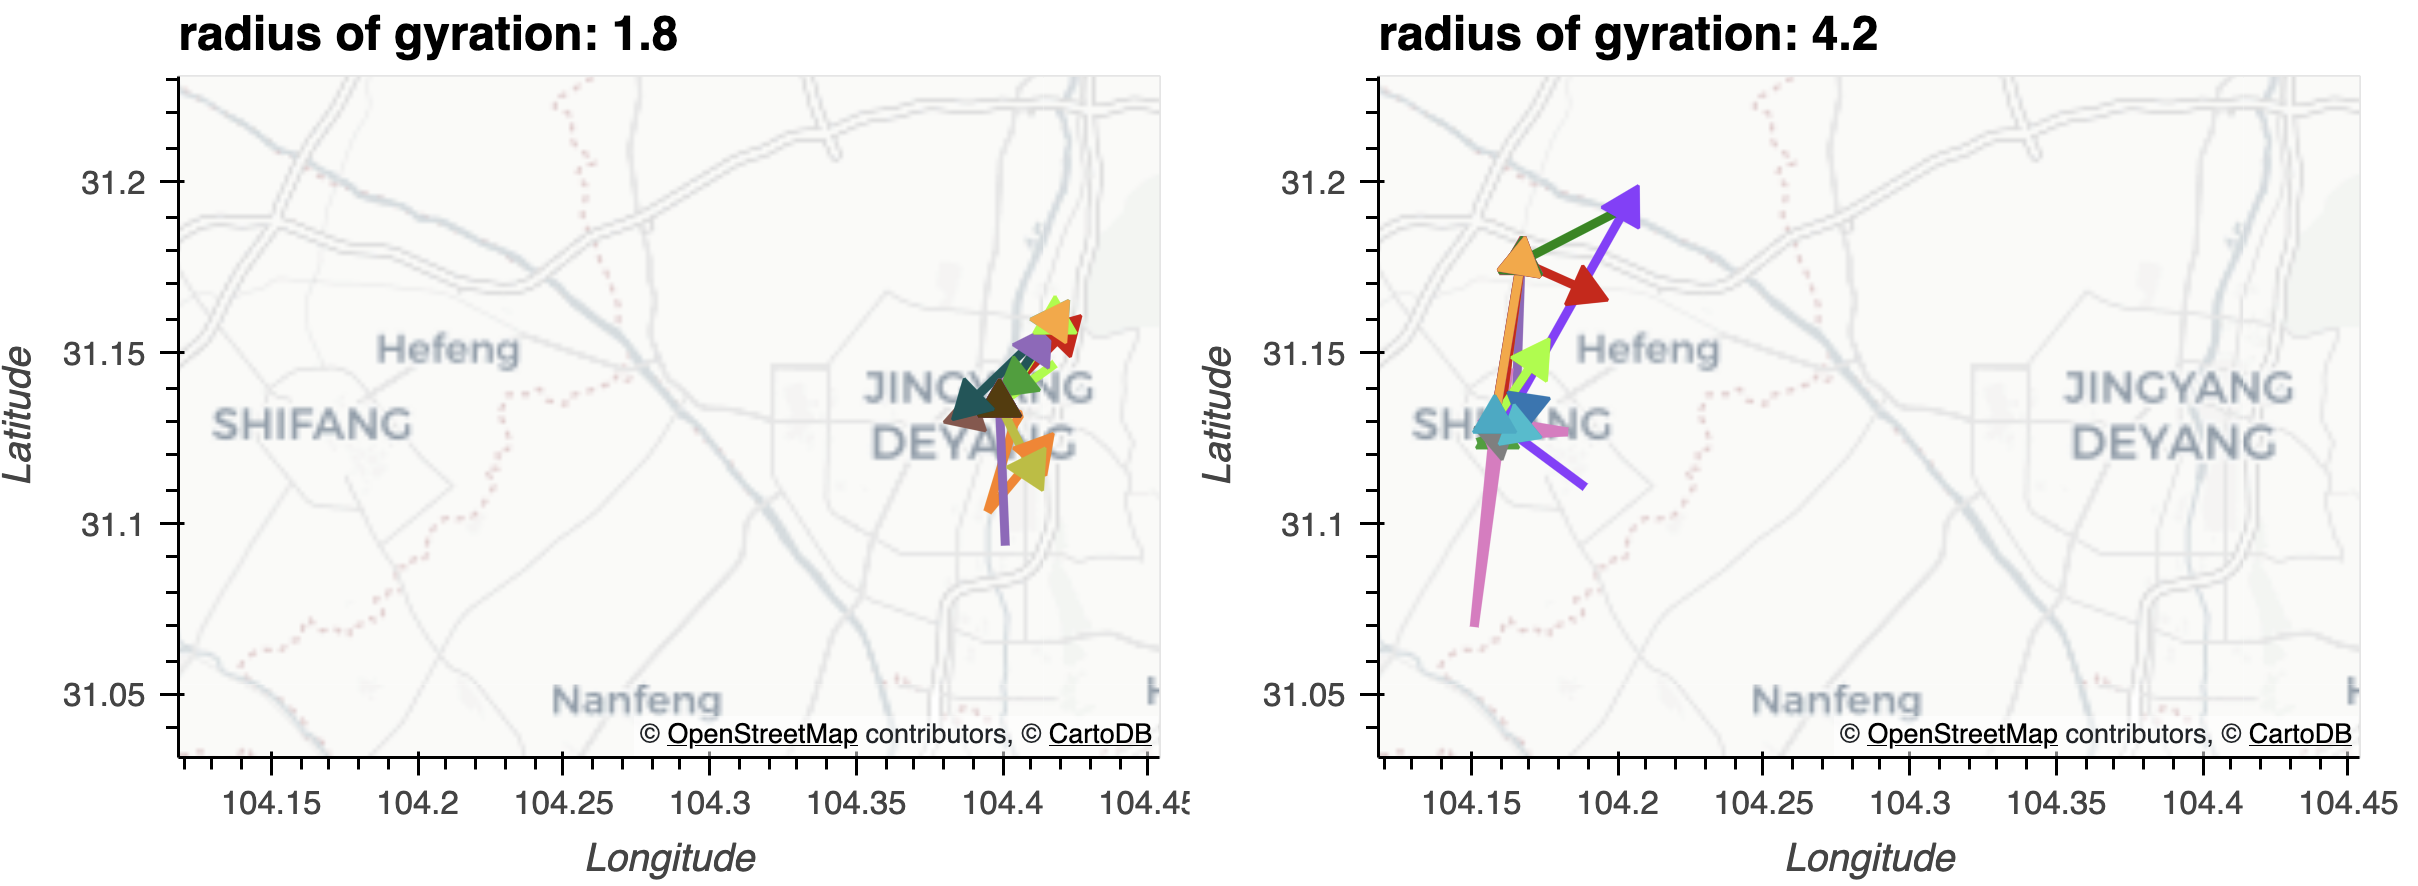
\includegraphics[width=1\textwidth]{figures/rg_compare.png}
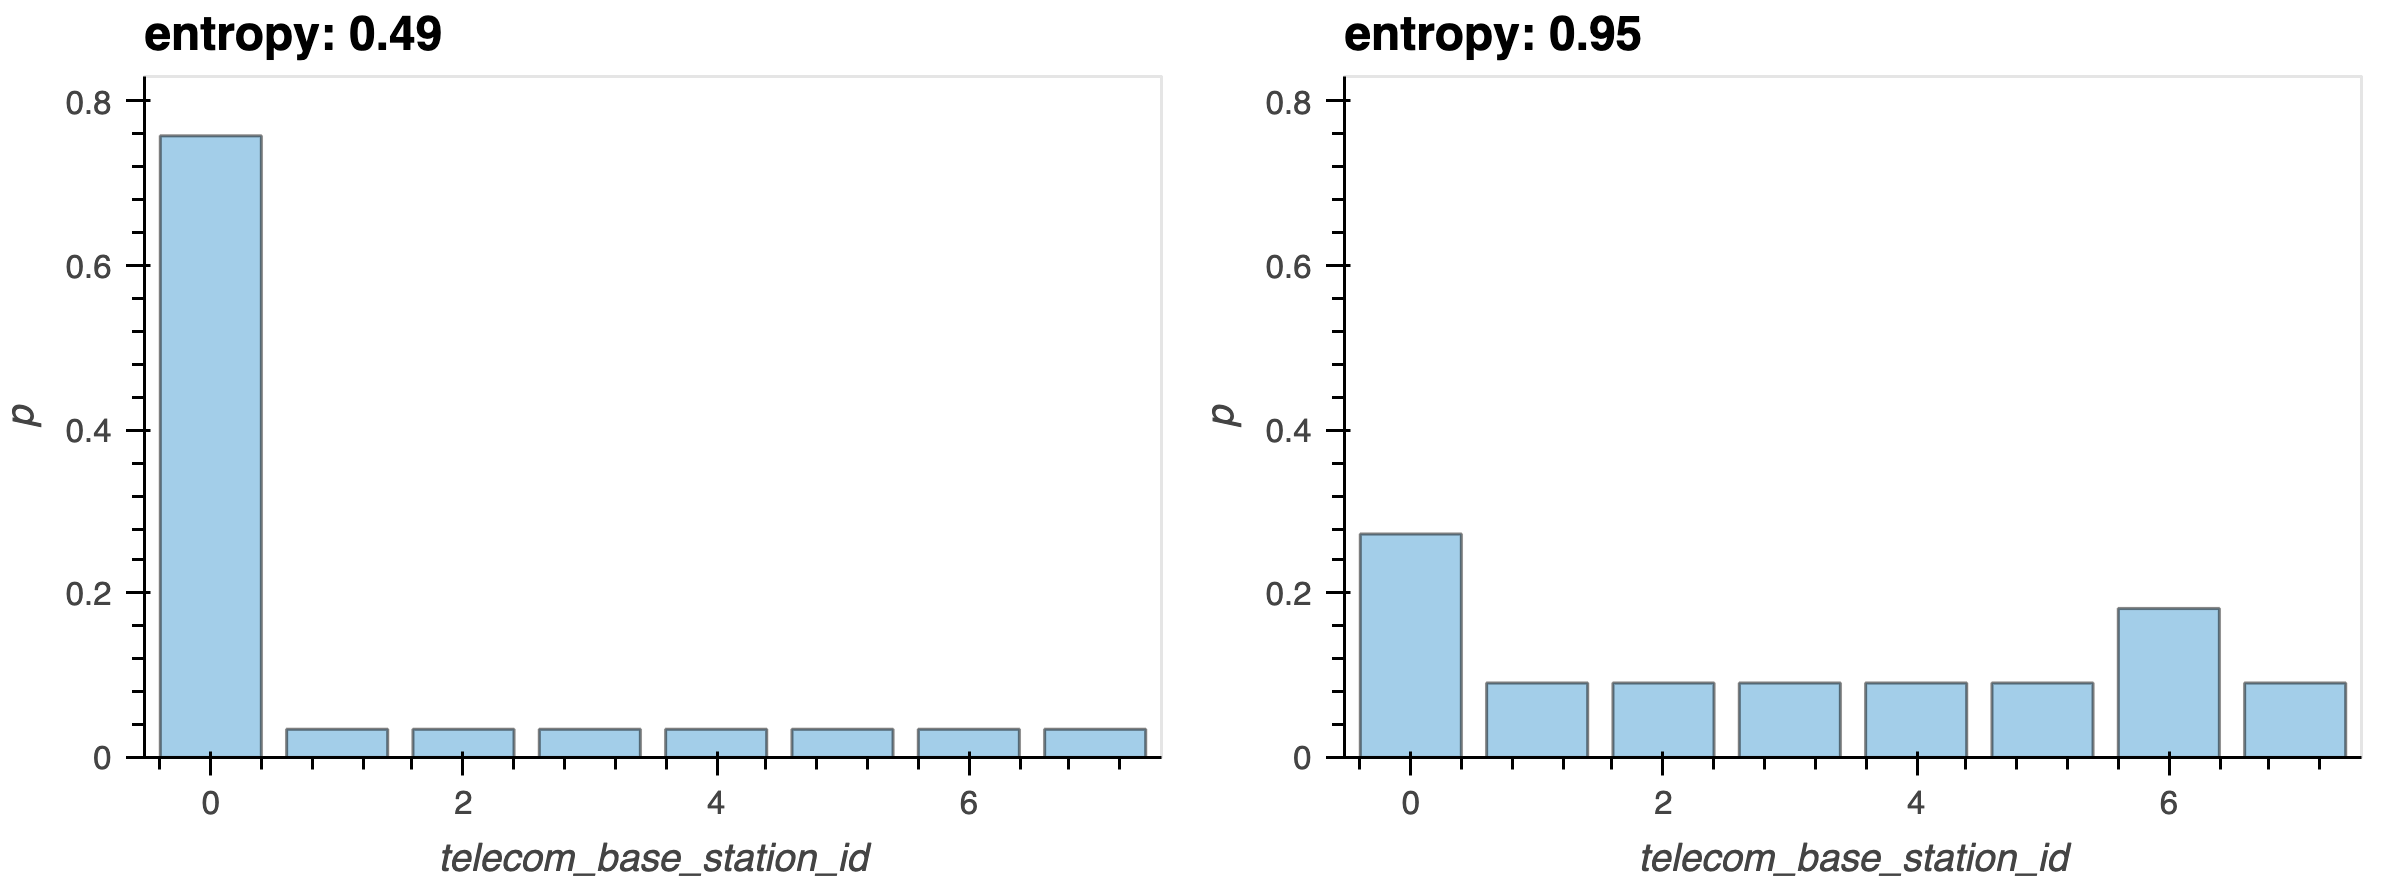
\includegraphics[width=1\textwidth]{figures/entropy_compare.png}
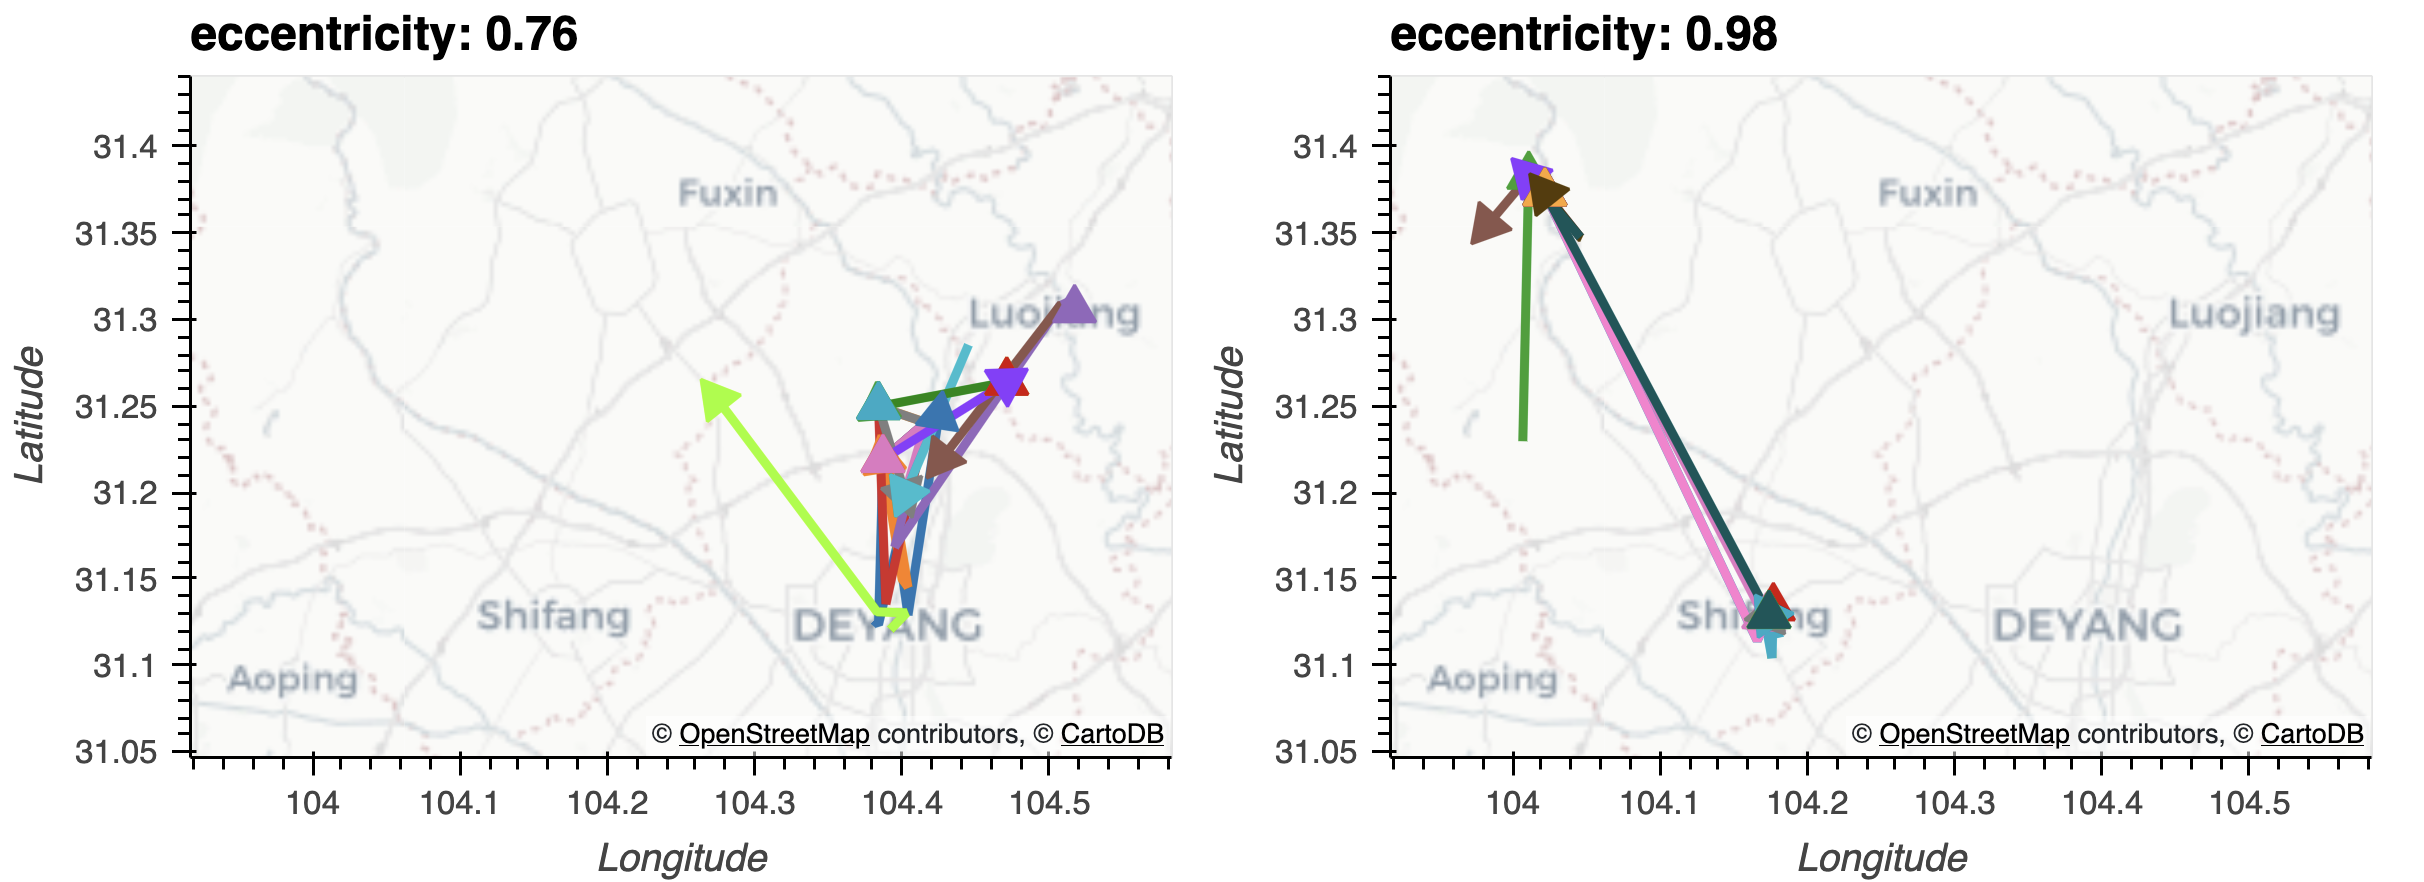
\includegraphics[width=1\textwidth]{figures/ecc_compare.png}

\vspace{0.1cm}
\caption*{Notes:  For radius of gyration and eccentricity, we visualize daily movement trajectories of four phone users throughout August 2013. Regarding entropy, we examine the distribution of telecom base station usage for two phone users during the same period, where the y-axis (p) represents the proportion of total days on which each base station was activated, calculated as the number of days a station served calls divided by the total number of such days across all stations.}
\label{fig:mobility}
\end{figure}

\vspace{0.3cm}
\begin{figure}[h!]
\centering
\caption{Visualization of Our Proposed Two-Staged Residential Location Estimation}
\vspace{0.1cm}

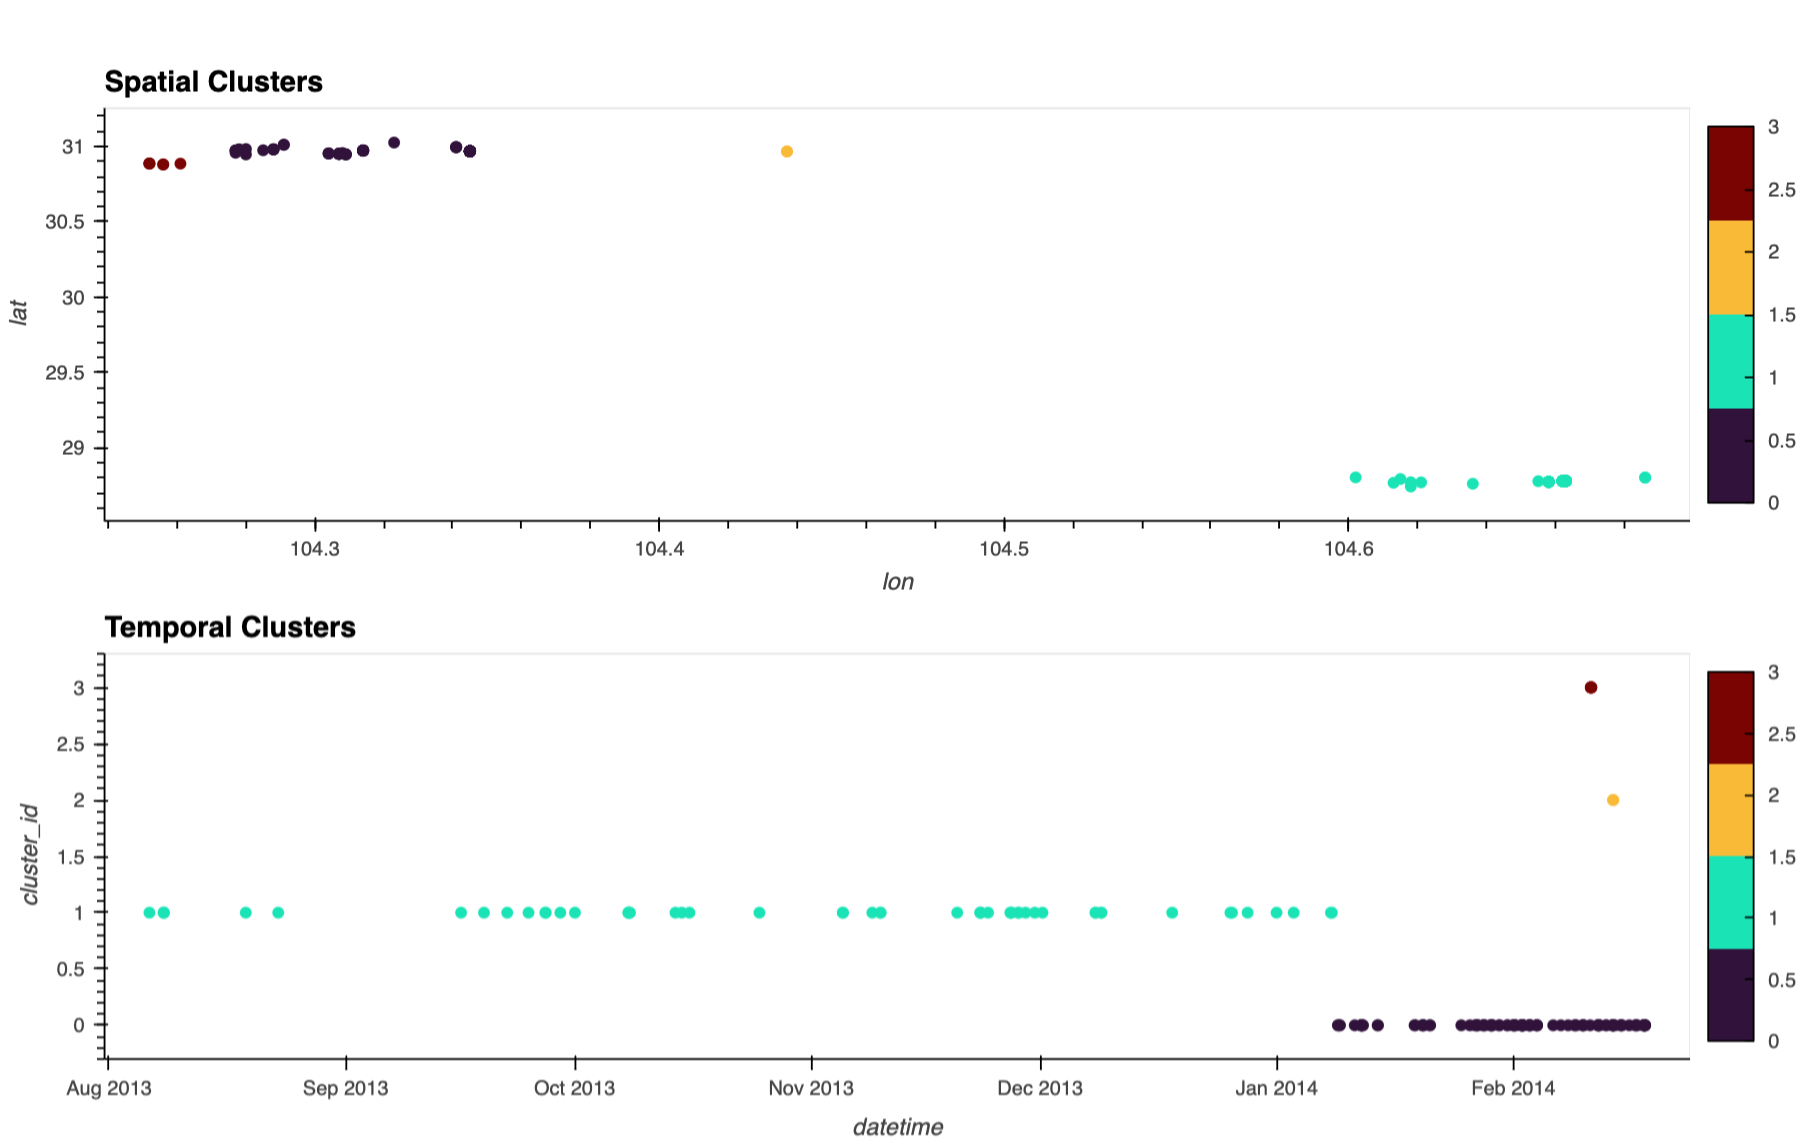
\includegraphics[width=1\textwidth]{figures/cluster_res.png}

\vspace{0.1cm}
\caption*{Notes:  This figure demonstrates one of the phone user's mobility patterns. The upper plot's x and y axis represent the longitude and latitude, respectively. The lower plot shows the temporal span of each cluster where the x axis represents the timestamp and the y axis represents the cluster index. The point is colored by the cluster index.}
\label{fig:cluster}
\end{figure}



We have three datasets: CDRs, coordinates of telecom base stations, and one that contains phone users' profile features, such as age, gender, phone brand, service type, etc. By joining CDRs with coordinates data on cell IDs, and then grouping by user phone numbers, we can obtain the daily history of movement trajectories of each phone user from August 2013 to May 2014. User profile data is uncommonly available due to privacy issues but critical for selecting samples of interest in our analysis. When constructing various mobility and mobile communication features or estimating residential coordinates, we want the samples to be consistently observable throughout the whole sample period, i.e., they don't cancel or register service in the middle of the sample period, to avoid spurious analysis due to too many missing records.

The cleaning of CDRs involves removing records where (i) either the calling or called number is not mobile phone numbers, (ii) either the start or end time is not valid timestamps, and (iii) the duration of calls is less than or equal to 0. For user profile data, we remove client numbers in profile data whose ID card numbers are not in the correct specification. After the cleaning, we have 0.5 to 0.6 billion call records per month and 348,241 client numbers whose profile features are available in each month.


\section{Notations}\label{sec:notations}
Denote $V$ as a set of the phone users, $B$ as a set of telecom base stations and $T = M \times D \times H$ as a set of timestamps where $M$ is a set of calendar months spanning from Aug 2013 to May 2014, $D := \{1, 2, ..., 31\}$ and $H$ is a set of all possibles times in a day.

\begin{definition}[Call Detailed Records]
CDRs denoted by $R$ is a collection of phone calls, which are 4-tuples, containing information of the caller, recipient, timestamp, and telecom base station that services the call. It's defined as:
$$
R := \{
  (i, j, t, b) \in V \times V \times T \times B
  \mid
  i \text{ calls } j \text{ at timestamp } t \text{ and }
  \text{the call is serviced by } b
\}.
$$
\end{definition}

\begin{definition}[A User's Nighttime Call Records Serviced by a Telecom Base Station]
Given CDRs $R$, we can filter call events that are either made or received by a user $i$ and serviced by a telecom base station $b$ during nighttime. Note that the definition of nighttime follows \cite{referral_effect_2023aer}. It's denoted by $R^{\text{night}}_{i, b}$ and defined as:
\begin{align*}
R^{\text{night}}_{i, b} := \{
    r \in R
    \mid
    &\text{there exists } t \in T \text{ where } t \geq \text{10 p.m.} \text{ and } t \leq \text{7 a.m.} \\
    &\quad \text{and } j \in V \text{ such that } r \in \{(i, j, b, t), (j, i, b, t) \}
 \}.
\end{align*}
\end{definition}

\begin{definition}[A Set of Timestamps of a User's Nighttime Call Records Serviced by a Telecom Base Station]
A subset $T^{\text{night}}_{i, b} \subset T$ is a collection of timestamps associated to $R^{\text{night}}_{i, b}$, and it's defined as:
$$
T^{\text{night}}_{i, b} :=
\{
    t \in T
    \mid
    \text{there exists } j \in V
    \text{such that either } (i, j, t, b) \text{ or } (j, i, t, b) \in R^{\text{night}}_{i, b}
\}.
$$
\end{definition}

\pagebreak
\begin{definition}[A Subset of Telecom Base Stations Connected to a User during Nighttime]
A subset $B^{\text{night}}_i \subset B$ of telecom base stations connected to a user $i \in V$ during nighttime is defined as:
\begin{align*}
B^{\text{night}}_i := \{
    b \in B
    \mid
    &\text{there exists } j \in V \text{ and } t \in T \\
    &\quad \text{such that either } (i, j, t, b) \text{ or } (j, i, t, b) \in R^{\text{night}}_{i, b}
\}.
\end{align*}
\end{definition}

\section{Spatial Clustering}
Recall that our estimation of residential locations consists of two stages and the first stage is to run the spatial clustering algorithm to aggregate the appearance patterns geographically during nighttime. A user $i$'s locations during nighttime are approximated by $B^{\text{night}}_i$, on which the clustering algorithm, DBSCAN, is applied. To be precise, location refers to an injective function $loc: B \rightarrow \mathbb{R}^2$ which maps each base station $b \in B$ to its geographic coordinates $loc(b) = (lon_b, lat_b)$ where $lon_b$ and $lat_b$ represent the longitude and latitude of telecom base station $b$, respectively. Our choice of DBSCAN is based on the fact that it does not require predefining number of clusters, unlike K-means, offering greater flexibility in identifying natural clusters within the data like CDRs.

Before applying DBSCAN, we need to decide the weight for each location $b \in B^{\text{night}}_i$, and we follow the idea of defining the weight of a base station as the number of days on which it services call records for user $i$ rather than the number of calls, which is borrowed from \cite{isaacman2011identifying} while they applied the clustering algorithm designed by \cite{hartigan1975clustering}. They argue that this approach can reduce the influence of base stations that were only used for a few days but had a burst of events on those days—for example, during a temporary vacation, people might make a lot of phone calls to share their experiences with their contacts. To enable this definition of weights for telecom base stations, we define a measure named as the temporal size over a set of timestamps that computes the number of unique days spanned by these timestamps. With the temporal size measure, the weight of a base station $b \in B^{\text{night}}_i$ is defined as the share of the temporal size related to $b$ to the aggregate temporal size across all $b \in B^{\text{night}}_i$.

\begin{function}[A Measure of Temporal Size of a Set of Timestamps]
The measure of temporal size of a subset $\tilde{T} \subset T$ of timestamps is defined as a measure  $\mu: 2^T \rightarrow \mathbb{N}$ where
\begin{equation}\label{eq:temporal_size}
\mu(\tilde{T}) =
|
\{
(m, d) \in M \times D
\mid
\text{there exists } h \in H \text{ such that } (m, d, h) \in \tilde{T}
\}
|.
\end{equation}
\end{function}

\label{def:temporal_size}
\begin{definition}[Telecom Base Station's Weight for a Client]
For a user $i \in V$ the weight for telecom base station $b \in B_i$ is defined as:
\[
w_i^{\text{night}}
:= \left\{
    w^{\text{night}}_{i, b} \in \mathbb{R}
    \mid
    w^{\text{night}}_{i, b} = \frac{\mu(T^{\text{night}}_{i, b})}{\sum_{b \in B^\text{night}_i} \mu(T^{\text{night}}_{i, b})}, b \in B^{\text{night}}_i
\right\}.
\]
\end{definition}

Thereafter, the distance measure between two locations is defined as $d: \mathbb{R}^2 \rightarrow \mathbb{R}$, which utilizes the Vincenty's formulae to compute the geographic distance (km) between two locations. For a user $i \in V$, we run the DBSCAN over $(\{\text{loc}(b)\}_{b \in B^{\text{night}}_i}, w^{\text{night}}_i)$ to obtain a set $C^{\text{night}}_i$ of clusters.

\begin{definition}[A Set of Nighttime Clusters of a Client]
\begin{align*}
C^{\text{night}}_i := \{
    C^{\text{night}}_{i, k} \subset B^{\text{night}}_i
    \mid
    &\text{for all } b_m, b_n \in C^{\text{night}}_{i, k}, \text{ where } m \neq n, d(\text{loc}(b_m), \text{loc}(b_n)) \\
    &\quad \text{meets DBSCAN neighbor criteria.}
\}.
\end{align*}
\end{definition}


\section{Estimation of Residential Location}\label{sec:estimation_of_residential_location}
\begin{figure}[h!]
\centering
\caption{Pipeline for Estimating A Phone User's Home Locations}
\vspace{0.1cm}

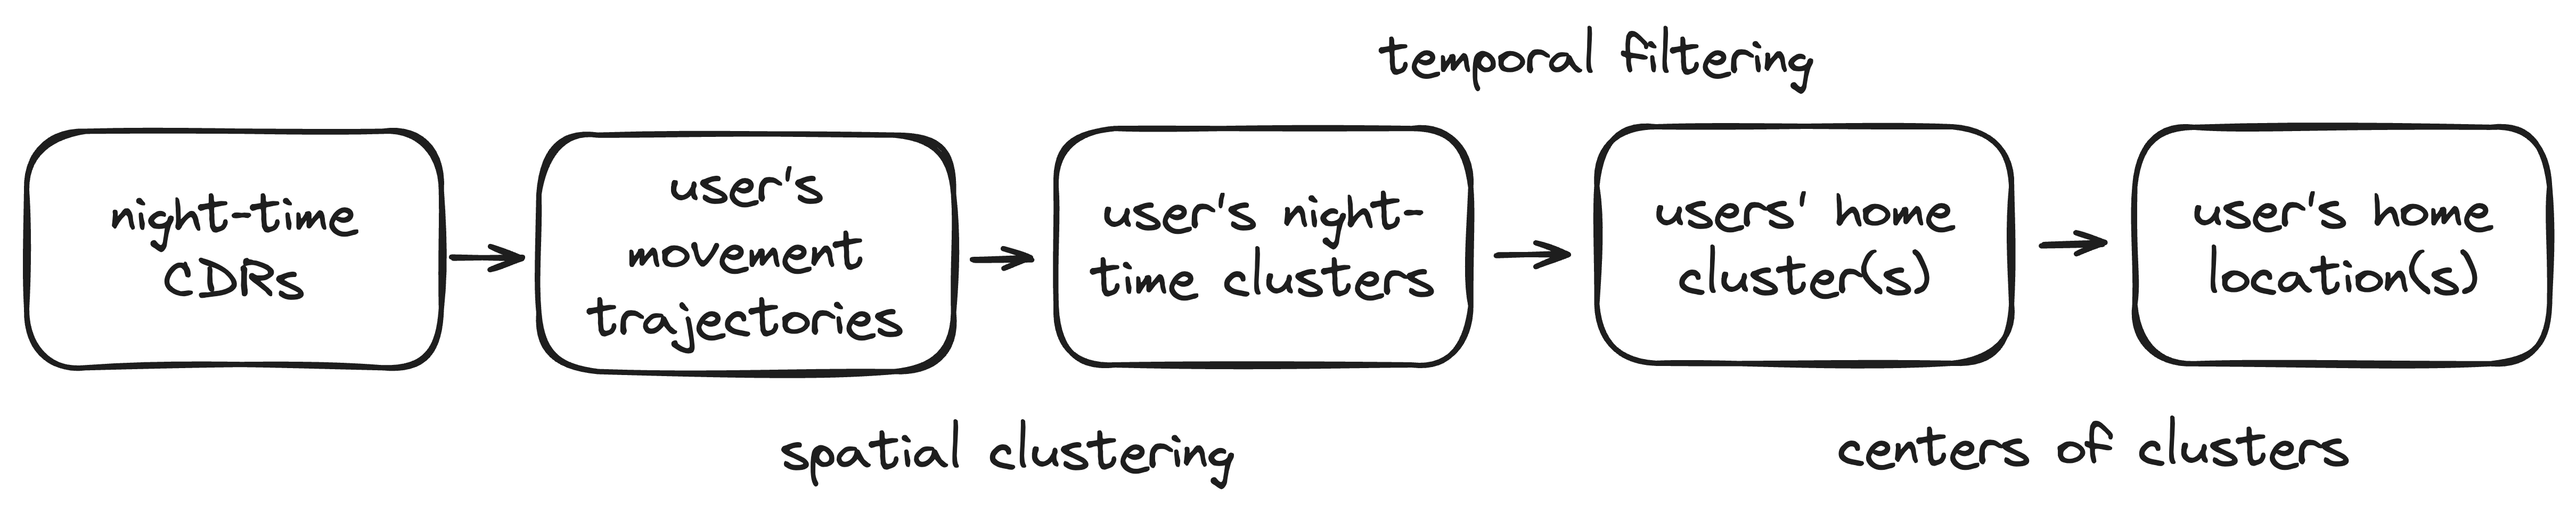
\includegraphics[scale=0.088]{figures/pipeline_home_locations.png}


% \caption*{Notes: .}
\label{fig:pipeline_home_location}
\end{figure}

This section aims at introducing how phone users' home locations are estimated, and Figure~\ref{fig:pipeline_home_location} presents all the steps for completing the task. After the procedure of spatial clustering, we can zoom out the level of spatial analysis from locations to clusters so the two issues arising from the routing mechanism are now resolved. Therefore, we define the new notations for both subsets of CDRs and timestamps based on $C^\text{night}_i$, which previously defined while considering $B^\text{night}_i$.

\begin{definition}[A User's Nighttime Call Records Serviced by a Nighttime Cluster]
For a cluster $C^{\text{night}}_{i, k}$ in $C^{\text{night}}_i$, a set of call records serviced by $C^{\text{night}}_{i, k}$ is defined as:
$$
\mathcal{R}^{\text{night}}_{i, k} := \bigcup_{b \in C^{\text{night}}_{i, k}} R^{\text{night}}_{i, b}.
$$
\end{definition}

\begin{definition}[A Set of Timestamps of a User's Nighttime Call Records Serviced by A Nighttime Cluster]
For a cluster $C^{\text{night}}_{i, k}$ in $C^{\text{night}}_i$, the timestamps of $\mathcal{R}^{\text{night}}_{i, k}$ is defined as:
$$
\mathcal{T}^{\text{night}}_{i, k} := \bigcup_{b \in C^{\text{night}}_{i, k}} T^{\text{night}}_{i, b}.
$$
\end{definition}

The second stage of the residential place estimation is to apply the temporal filtering trick, aiming at obtaining the home clusters, which contains a user's home locations. As mentioned in the introduction, eligible home clusters should be those that service the calls on the most number of days during a time period. Moreover, people might change their home locations during the sample period, and the home clusters afterward should also satisfy the definition of home clusters and the pre-moving period shouldn't overlap with the post-moving period.

Before defining the overlap, we need to define objects associated to two distinct clusters that can be identified to be overlapping with each other. The object is the service time intervals, which are continuous time intervals starting from the first time that a cluster services calls and ending at the last time that a cluster services calls.

\begin{function}[The First \& Last Timestamp of a Set of Timestamps]
Consider a set of timestamps $\tilde{T} \subset T$, the first and the last timestamps of which can be obtained by the following functions.
$$
t^{\text{first}}: 2^{T} \rightarrow T, \quad t^{\text{first}}(\tilde{T}) = \min_t \{t \in \tilde{T}\}.
$$
$$
t^{\text{last}}: 2^{T} \rightarrow T, \quad t^{\text{last}}(\tilde{T}) = \max_t \{t \in \tilde{T}\}.
$$
\end{function}

\begin{definition}[A Nighttime Cluster's Service Time Interval]
A continuous time interval associated to a nighttime cluster $C^{\text{night}}_{i, k} \in C^{\text{night}}_i$ is defined as: $[t^{\text{first}}(\mathcal{T}^{\text{night}}_{i, k}), t^{\text{last}}(\mathcal{T}^{\text{night}}_{i, k})]$, which represents that the cluster $C^{\text{night}}_{i, k}$ services nighttime phone calls for client $i$ during this period.
\end{definition}

\begin{definition}[Temporal Overlappness between Two Nighttime Clusters]
Consider two nighttime clusters, $C^{\text{night}}_{i, 1}, C^{\text{night}}_{i, 2}$, they overlap with each other temporally means there exists $t \in T$ such that $t$ is in both service time intervals of $C^{\text{night}}_{i, 1}$ and $C^{\text{night}}_{i, 2}$.
\end{definition}

With the definition of overlap, our temporal filtering trick is a sequential process, where we first sort the clusters in $C^{\text{night}}_i$ in descending order by the temporal sizes defined by $\mu(\mathcal{T}^{\text{night}}_{i, k})$ where $C^{\text{night}}_{i, k} \in C^{\text{night}}_i$, and then we iteratively select the cluster to be the home cluster that is not temporally overlap with any of the pre-selected home clusters. Note that the first home cluster is the cluster with the largest temporal size. The algorithm is shown in Algorithm \ref{home_cluster} and the complexity analysis is in Appendix A. Note that at the last step of the algorithm, the home clusters' start times of service time intervals are well-defined based on the corresponding nighttime clusters.

\begin{algorithm}[h!]
    \renewcommand{\algorithmicrequire}{\textbf{Input:}}
    \renewcommand{\algorithmicensure}{\textbf{Output:}}
    \caption{Home Cluster Estimation}
    \label{home_cluster}
    \begin{algorithmic}[1]
        \REQUIRE $C^\text{night}_i$
        \ENSURE $C^\text{home}_i$

        \STATE $\text{candidates} \leftarrow$ sort $C^\text{night}_i$ in descending order by the temporal size
        \STATE $C^\text{home}_i \leftarrow [\text{candidates}[1]]$
        \STATE

        \FORALL {$j=2,\cdots,\text{length}(\text{candidates})$}
            \STATE $\text{isolate} \gets \text{true}$
            \STATE $\text{candidate} \gets \text{candidates}[j]$
            \STATE

            \FORALL {$k=1,\cdots,\text{length}(C^\text{home}_i)$}
                \IF {$\text{candidate}$ temporally overlaps with $C^\text{home}_i[k]$}
                    \STATE $\text{isolate} \gets \text{false}$
                    \STATE \textbf{break}
                \ENDIF
            \ENDFOR
            \STATE

            \IF {$\text{isolate} = \text{true}$ and the temporal size of candidate $> 2$}
                \STATE insert $\text{candidate}$ into $C^\text{home}_i$
            \ENDIF
        \ENDFOR
        \STATE

        \STATE sort $C^\text{home}_i$ in ascending order by the start time of service time interval
        \STATE \textbf{return} $C^\text{home}_i$
    \end{algorithmic}
\end{algorithm}

Given the home clusters, we can define the home locations as the centroids of clusters, computed by the weighted average of the locations of the base stations in the cluster, where the weights are the temporal sizes.

\clearpage\newpage
\begin{definition}[A User's Home Location]
For a user $i \in V$, the $l$-th home location $(r_c)^{\text{home}}_{i, l}$ is defined by the weighted average over locations $\{\text{loc}(b)\}_{b \in C^{\text{home}}_{i, l}}$ of telecom base stations that are contained in the $l$-th home cluster $C^{\text{home}}_{i, l}$ where the weights are defined based on the temporal sizes $\{w^{\text{night}}_{i, b}\}_{b \in C^{\text{home}}_{i, l}} \subset w^\text{night}_i$. Below is the formula:
$$
(r_c)^{\text{home}}_{i, l} =
\sum_{b \in C^{\text{home}}_{i, l}}
\tilde{w}^{\text{night}}_{i, b} \text{loc}(b)
$$
where $\tilde{w}^{\text{night}}_{i, b} = \frac{w^{\text{night}}_{i, b}}{\sum_{b \in C^{\text{home}}_{i, l}} w^{\text{night}}_{i, b}}$.
\end{definition}

\section{Identification of Residential Shift and Its Timing}\label{sec:identification_of_residential_shift}
Residential shift is identified if a user's home location changes.
% As we aim to assess whether the residential shift will affect individuals' mobility and mobile communication patterns, and if effects are confirmed, how they evolve over time, the difference-in-differences (DiD) framework is appropriate in that we can recover the average treatment effect on the treated (ATT) for each post-treatment period under the parallel trend assumption.  Note that the treatment refers to the residential shift. ATT aims at quantifying the difference between the observed outcome of the treatment group and the potential outcome if they have never been treated. ATT aligns with our research questions in that the effect of residential shift functions on migrants' mobility and mobile communication patterns, potentially causing them to deviate from those associated with the case where migrants have never migrated.
Since CDRs record users' locations discretely and irregularly, it's ambiguous to decide the migration timing, as there may be latency between the actual date where users relocate and the date of the first timestamp where the second home cluster serves the calls. The determination on the migration timing is crucial in the design of the DiD with multiple periods as it determines the pre-treatment and post-treatment periods where the parallel trend assumption is tested, and the treatment effect dynamics are inspected, respectively.

At first thought, we can define the migration timing as (i) the date of the last timestamp where the first home cluster serves the calls, (ii) the date of the first timestamp where the second home cluster serves the calls, or (iii) the date in the middle of them. We opt for a conservative approach and select the second option, which guarantees that the chosen date occurs after migration has already been completed. This decision results in the necessity to consider the violation of "no anticipation" (\cite{callaway2021difference}, \cite{sun2021estimating}, \cite{borusyak2024revisiting}) because people might start to collect information for better preparation before migrating to another prefecture, causing the divergent paths of mobility and mobile communication features between migrants and non-migrants before a actual migration event takes place. Note that the no anticipation assumption doesn't require hold in all pre-treatment periods; instead, it's plausible to assume it holds until a period before the treatment.

Conventionally, the discussions on treatment effect dynamics are on a yearly basis; however, we are discussing treatment effect dynamics on a monthly level from August 2013 to May 2014. Therefore, to establish clean notations, we index the monthly periods from integer 1 to 10 where August 2013 corresponds to $1$, September 2013 corresponds to $2$, and so on. Furthermore, we denote $\mathcal{M} := \{1, \cdots, 10\}$ as the set of monthly periods after indexing. Below we define the treatment group consisting of four subgroups $\{ \mathcal{G}_g \}_{g=4,5,6,7}$ as migrants who relocate in different months $g$ and define the never-treated group $\mathcal{G}_{\infty}$ as non-migrants. We utilize the symbol $\infty$ to indicate a non-migrant will relocate in the far-away future, i.e., infinity period (\cite{sun2021estimating}, \cite{borusyak2024revisiting}).

\begin{definition}[Migrants]\label{def:migrants}
A phone user $i \in V$ is a migrant associated with the group $\mathcal{G}_g$ if (i) user $i$ only changes home locations once during the sample period, (ii) the two home locations are in different prefectures, and (iii) the migration event occurs in month $g \in \{4,5,6,7\} \subset \mathcal{M}$.
\end{definition}

\begin{definition}[Non-Migrants]
A phone user $i \in V$ is a non-migrant associated with the group $\mathcal{G}_{\infty}$ if $i$ doesn't change the home locations throughout the sample period.
\end{definition}

We require migrants to have only relocated once because among users who have multiple residential shifts, most of them have only gone through it once, accounting for 99.65\%. Besides, targeting these users can provide more pre-treatment periods for each residential shift, thereby making the parallel trend assumption easier to test.

Longer distance migration should be more likely to have substantial impacts on mobility and mobile communication patterns so we restrict our discussions on inter-prefecture migrants. As Table \ref{tab:migration_sample} demonstrates, we don't lose too many migrants by restricting the definition of migrants to those crossing prefectures.

\begin{table}[htbp]
\vspace{0.2cm}
\renewcommand{\arraystretch}{1.6}
\setlength{\tabcolsep}{4mm}{}
\centering
\small
\caption{Statistics of Migrants by the Month of Migration}
\begin{tabular}{lcccccc} \hline
& \multicolumn{3}{c}{Count of Migrants} & \multicolumn{3}{c}{Migration Distance} \\
\cline{2-4} \cline{5-7}
month & all & inter-pref. & ratio (\%) & all & inter-pref. & ratio (\%) \\ \hline
Aug. 2013 & 2434 & 2006 & 82.42 & 134.8 & 157.11 & 116.55 \\
Sep. 2013 & 974 & 797 & 81.83 & 135.82 & 159.25 & 117.25 \\
Oct. 2013 & 451 & 311 & 68.96 & 119.01 & 158.83 & 133.46 \\
Nov. 2013 & 363 & 247 & 68.04 & 101.0 & 137.35 & 135.99 \\
Dec. 2013 & 305 & 231 & 75.74 & 132.15 & 164.7 & 124.63 \\
Jan. 2014 & 448 & 338 & 75.45 & 128.04 & 160.78 & 125.57 \\
Feb. 2014 & 594 & 458 & 77.1 & 116.56 & 142.44 & 122.2 \\
Mar. 2014 & 594 & 443 & 74.58 & 118.48 & 148.91 & 125.68 \\
Apr. 2014 & 675 & 519 & 76.89 & 129.55 & 160.28 & 123.72 \\
May 2014 & 1520 & 1222 & 80.39 & 127.37 & 151.29 & 118.78 \\
\hline
\end{tabular}
\label{tab:migration_sample}%
\end{table}%

\vspace{-2.5em}
\begin{singlespace}
\begin{footnotesize}
\noindent Notes: The column all represents the count of migrants and migration distance are computed on the phone users who satisfy the first requirement of migrants. Therefore, they don't necessarily change their home locations to another prefecture. The column, inter-pref., means statistics are computed on the phone users who satisfy the first and second requirement of migrants. Moreover, the unit of distance is in kilometers.
\end{footnotesize}
\end{singlespace}

The treatment timing varies across users who have once changed their residential locations, but we select those who migrate in the middle of the sample period, i.e., $g \in \{4,5,6,7\}$. For these users, we have higher confidence level to safely classify them as migrants in that the temporal sizes of the two home clusters are comparable. For example, if the residential shift takes place in September 2013, then the first cluster's temporal size is about a month while the second cluster's temporal size is very likely to be greater than a month with a maximum of 9 months. In this case, the two home clusters are obviously not comparable in terms of the temporal sizes, so we are less confident to classify this user as a migrant because the first cluster may be a short visit, and the first timestamp associated with the second home cluster might be even earlier, outside the sample period. Referring to Table \ref{tab:migration_sample}, it seems that there are many users relocating in the early and late period of the sample period, highlighting the importance to restrict the definition of migrants to those relocate in the middle of the sample period. Besides, restricting migrants to those who relocate in the middle of the sample period doesn't substantially distort the origin-destination distribution, as the KL-divergence is about 0.35, which is calculated by comparing the origin-destination distribution of inter-prefecture migrants who migrate in the middle of the sample period to that of migrants who migrate in all months.

We can define some parameters to rule out users who have incomparable temporal sizes of home clusters, for example, requiring the temporal sizes of the home clusters or even the ratio between them to be greater than thresholds. Nonetheless, as aforementioned, it's not necessary to define such parameters. We can simply follow the patterns of the data and conduct restrictive sample selection to validate the robustness of the results. Moreover, even if these parameters are defined, they are not employed to reduce methodological error—like other existing methods to identify residential shift mentioned in section 1.5—rather, it's a decision on how much we should trust the patterns

% \textbf{Q: What the difference between the complete migrant sample and subsample?}

Table \ref{tab:non_migrant_migrant_comparison} presents the sample statistics of our final selection on migrants, compared to the non-migrant groups.
We can see that migrants' characteristics differ slightly between the complete migrant sample and the subsample including only those who migrate in the middle of sample period.
The differences in demographic features compared to non-migrants are larger for the subsample migrants than for the complete migrant sample, while the differences in phone-related characteristics compared to non-migrants are smaller for the subsample migrants.

% \textbf{Q: What the difference between the migrants and non-migrants?}

Examining Panel B more closely, as we define the treatment group for analysis as those who migrate across prefectures during the middle of the sample period.
Compared to non-migrants, these migrants tend to be younger and have a higher probability of being male, with a lower likelihood of being born in Deyang city.
Furthermore, they own slightly better phone devices and a higher fraction of them use smartphones.
% but they have approximately the same number of phones as non-migrants.revealed by the data.

\begin{table}[htbp]
\vspace{0.2cm}
\renewcommand{\arraystretch}{1.6}
\setlength{\tabcolsep}{1mm}{}
\centering
\small
\caption{Comparison of Non-Migrant and Migrant Statistics}

\begin{tabular}{lcccc} \hline
Variable & Non-Migrant & Migrant & Difference & p-value \\ \hline
\textit{Panel A: Inter-Prefecture Migrants, Any} \\
age & 40.87 & 36.67 & -4.2 & 0.0 \\
male flag & 0.66 & 0.68 & 0.02 & 0.0001 \\
born in Deyang flag & 0.82 & 0.65 & -0.17 & 0.0 \\
(max) phone price & 954.72 & 1059.87 & 105.15 & 0.0 \\
(max) smartphone flag & 0.65 & 0.77 & 0.12 & 0.0 \\ \hline

\textit{Panel B: Inter-Prefecture Migrants, Middle Period} \\
age & 40.87 & 35.56 & -5.31 & 0.0 \\
male flag & 0.66 & 0.71 & 0.05 & 0.0001 \\
born in Deyang flag & 0.82 & 0.61 & -0.21 & 0.0 \\
(max) phone price & 954.72 & 1011.0 & 56.28 & 0.0234 \\
(max) smartphone flag & 0.65 & 0.74 & 0.09 & 0.0 \\ \hline

\end{tabular}

\label{tab:non_migrant_migrant_comparison}%
\end{table}%

\vspace{-2em}
\begin{singlespace}
\begin{footnotesize}
\noindent Notes: (i) Panel A presents statistics for phone users who meet the first two requirements of the migrant definition outlined in Definition \ref{def:migrants} without restricting the migration timeframe, while Panel B analyzes data based on the complete migrant definition, limiting inter-prefecture migrants to those who migrated between November 2013 and February 2014. (ii) The variables include: male flag, a binary indicator of user gender; born in Deyang flag, a binary variable indicating whether the user was born in Deyang prefecture; and (max) phone price, and (max) smartphone flag, which are time-variant variables constructed using data before November 2013 to examine pre-treatment covariates. (iii) Since phone users may have changed devices or own multiple phone devices between August 2013 and October 2013,(max) phone price represents the highest price among all phones a user owned during this period, and (max) smartphone flag indicates whether a user ever owned a smartphone during this period.
\end{footnotesize}
\end{singlespace}



% As the treatment is staggered in adoption and heterogeneous treatment effects are plausible over time or across treatment-timing groups, we will apply the estimation approach proposed by \cite{callaway2021difference} to avoid the problematic estimation on treatment effect. As they point out, the treatment effect dynamics can be correctly identified in the setting of variable treatment timing, only if the composition of the treatment group is fixed. Therefore, up to 4 post-treatment periods' differences in treatment effect can be easily interpreted as the treatment effect dynamics because for migrants who migrate in month 5 (February 2014), the fifth post-treatment period, June 2014, outcomes are missing, leading to the change in the composition of treatment-timing group.

\clearpage\newpage
\section{Detection of Smartphone Adoption}
Aside from residential shifts, our user information data enables us to inspect the effects of other shift events, specifically upgrading to smartphones. Smartphones have abundant functionalities that facilitate mobile communication and better assist users in exploring unfamiliar environments through GPS technology, potentially altering smartphone adopters' mobility patterns. To study the smartphone-adoption shift, we define the treated and untreated units as follows.

\begin{definition}[Smartphone Adopters]\label{def:smartphone_adopter}
A phone user $i \in V$ is a smartphone adopter associated with group $\mathcal{G}_g$ if user $i$ (i) changes from a non-smartphone device to a smartphone model, (ii) is not observed to switch back to non-smartphone devices throughout the sample periods, and (iii) the adoption event occurs in month $g \in \{4,5,6,7\} \subset \mathcal{M}$, where these months represent the middle of the sample period.
\end{definition}

This definition rules out phone users who have multiple cellphones, and constantly switch between smartphone and non-smartphone devices.
As defining migrants, we require the events to happen in the middle of the sample period to confirm the reliability of the adoption event, avoiding the observation window bias.
Besides, there are also more periods left for us to inspect the ATT dynamics.

\begin{definition}[Non-Smartphone Users]
A phone user $i \in V$ is a non-smartphone user associated with group $\mathcal{G}_{\infty}$ if user $i$ consistently uses non-smartphone devices throughout the sample periods.
\end{definition}

We reuse the notations: \( \mathcal{G}_g \) and \( \mathcal{G}_{\infty} \) to denote the treated and non-treated cohorts.

\begin{figure}[h!]
\centering
\caption{Number of Phone Users Upgrading to Smartphones by Month}
\vspace{0.1cm}

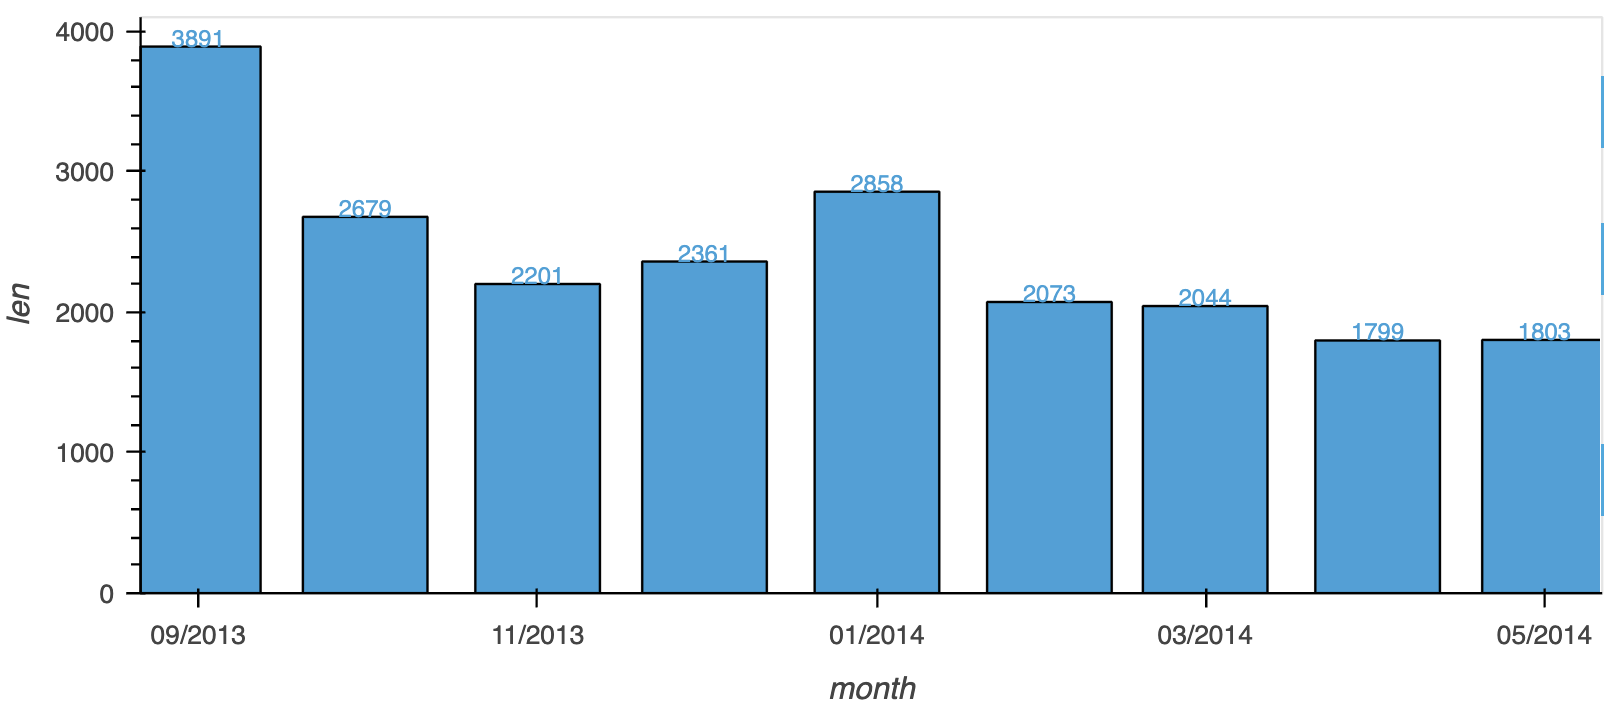
\includegraphics[scale=0.51]{figures/number_of_smartphone_adopters.png}


% \caption*{Notes: .}
\label{fig:number_of_smartphone_changers}
\end{figure}

The above figure shows the counts of smartphone adopters for each month. Generally, there are few differences across months, except a notable increase in September 2013, owing to the observation window bias.

\begin{table}[htbp]
\vspace{0.5cm}
\renewcommand{\arraystretch}{1.6}
\setlength{\tabcolsep}{1.1mm}{}
\centering
\small
\caption{Comparison of Smartphone Adopters to Non-Smartphone Users Statistics}
\begin{tabular}{lcccc} \hline
Variable & Non-Changers & Changers & Difference & p-value \\ \hline
\textit{Panel A: Smartphone Adopters, Any} \\
age & 44.7 & 41.68 & -3.02 & 0.0 \\
male flag & 0.66 & 0.65 & 0.0 & 0.5039 \\
born in Deyang flag & 0.86 & 0.83 & -0.03 & 0.0 \\
(max) phone price & 409.9 & 706.11 & 296.22 & 0.0 \\ \hline

\textit{Panel B: Smartphone Adopters, Middle Periods} \\
age & 44.7 & 41.84 & -2.86 & 0.0 \\
male flag & 0.66 & 0.66 & 0.0 & 0.8563 \\
born in Deyang flag & 0.86 & 0.83 & -0.02 & 0.0 \\
(max) phone price & 409.9 & 501.75 & 91.85 & 0.0 \\ \hline

\end{tabular}
\label{tab:non_changer_changer_comparison}%
\end{table}%

\vspace{-2em}
\begin{singlespace}
\begin{footnotesize}
\noindent Notes: (i) The Changers refers to the smartphone adopters and non-changers mean non-smartphone users. (ii) The Panel A compares pre-treatment covariates between smartphone adopters (upgrading in any month) and non-smartphone users. Panel B examines the same comparison but restricts smartphone adopters to those upgrading between November 2013 and February 2014. (iii) The pre-treatment covariates are crafted in the same way with Table \ref{tab:non_migrant_migrant_comparison}.
\end{footnotesize}
\end{singlespace}


\clearpage\newpage
Table~\ref{tab:non_changer_changer_comparison} shows that smartphone adopters who upgrade during middle periods are largely similar to those upgrading during any month of the sample period, with the exception of owning slightly less expensive devices.
This pattern may result from observation window bias.
Panel A includes users who switch to smartphones during early sample periods, but we lack sufficient observation periods to verify their consistent use of non-smartphone devices before adoption.

The definition of "changers" in Panel B of Table~\ref{tab:non_changer_changer_comparison} corresponds to our  formal definition of smartphone adopters presented in Definition~\ref{def:smartphone_adopter}.
We can see that smartphone adopters are slightly younger, marginally more likely to be born outside Deyang prefecture (by approximately 2\%), and own more expensive non-smartphone phone devices (before adoption) compared to non-smartphone users.
Besides, the age composition of the two groups shows no significant difference.

\clearpage\newpage
\section{Construction of Outcome Variables}
Our outcomes of interest contain two groups: mobile communication and human mobility features.
For each group, we craft three kinds of features to study the effects of residential shift and smartphone adoption on these outcome variables.

Mobile communication network features are derived from the reciprocated network and include three kinds of features: call duration, contact entropy, and contact distance.
The contact distance isn't commonly seen in the related literature, but it contains rich interpretations of how phone users' mobile communication network geographies look. Besides, it's more complicated to construct compared to the other two as it can't be directly derived from the call detailed records.
Instead, we need a preliminary home-estimation procedure, then compute the average geographical distance between a phone user's home and the other contacts' homes.
Therefore, it serves as a great extension of our robust home estimation method presented in Section~\ref{sec:estimation_of_residential_location}.

Mobility features consist of radius of gyration, movement entropy, and eccentricity. Jointly considering movement entropy and eccentricity offers additional insights, beyond the "unpredictability" provided by movement entropy alone. Specifically, we can identify distinct mobility patterns, such as whether users exhibit highly random movements that are stretched along one direction (high entropy, high eccentricity) versus more predictable movements that spread evenly across all directions (low entropy and low eccentricity). We will see interesting evolution in these patterns after migration and upgrading to smartphone devices.

What's more, entropy-based variables can be viewed as measures of diversity, in addition to unpredictability.
Employing entropy as a measure of diversity captures another aspect beyond quantity increases, e.g., interacting with more friends or visiting more places.
Entropy says diversity should also be credited to the randomness. That is, calling the same number of friends with equal frequency demonstrates a sign of diversity.
Besides, we can measure the diversity while eliminating the variation in quantity by normalizing it (dividing by \( \log(N) \), where \( N \) can be the total number of contacts/locations).

\subsection{Mobile Communication Network Features}
We haven't formally defined what the mobile communication network is. Basically, the nodes of the network are defined as phone users and edges are defined as reciprocated calls that occur on weekdays, which are further defined as follows.

\begin{definition}[A Reciporated Call]
A call record $r \in R$ where $r = (i, j, t, b)$ for some $i, j \in V, t \in T$ and $b \in B$ is reciprocated if there exists $t' \in T$ and $b' \in B$ such that $(j, i, t', b') \in R$.
\end{definition}

Note that the mobile communication network is a kind of directed network---i.e., for example, a user $i$ calls $j$ and $j$ calls $i$ are considered as two edges, whereas this would be considered as a single edge in an undirected graph. Besides, the edges are weighted by the underlying call duration (in minutes). Since mobile communication is directed, we can naturally build relevant features based on distinct communication directions.
To avoid redundantly defining the same features for both incoming and outgoing calls, we will illustrate the feature definitions using outgoing calls as examples.

After constructing the mobile communication network by month, directional call duration for a user \( i \in V \) in a given month \( m \in \mathcal{M} \) is computed by separately aggregating incoming and outgoing calls' duration.
Contact entropy is constructed based on the Shannon entropy normalized by the logarithm of the number of contacts for a user $i$ in a given month $m$.
Normalization is necessary as it accounts for differences in network size across phone users, thereby leading to clearer interpretation of the regression coefficients.
Intuitively, increasing unnormalized entropy by 0.3 doesn't mean the same thing for a user with 10 friends versus one with 50 friends.

\begin{definition}[Outgoing Contact Entropy]
The outgoing contact entropy $ce^{\text{out}}_{i,m}$ (where $ce$ stands for contact entropy) for user $i$ in month $m$ is defined by:
\[
ce^{\text{out}}_{i,m}
=
\frac
{-\sum_{j \in V^{\text{out}}_{i,m}}
\hat{p}_{i,j,m} \log(\hat{p}_{i,j,m})}{\log(\lvert V^\text{out}_{i, m} \rvert )}
\]
where
\begin{equation}\label{eq:outgoing_contacts}
V^{\text{out}}_{i,m}
:=
\{
j \in V
\mid
\text{user } i \text{ has once called user } j \text{ in month } m
\}
\end{equation}
and
\begin{equation}\label{eq:weight_j_for_i_in_month_m}
\hat{p}_{i,j,m}
= \frac{w_{i,j,m}}{\sum_{k \in V^{\text{out}}_{i,m}} w_{i,k,m}}
\end{equation}
with $w_{i,j,m}$ being the weight of edge from user $i$ to user $j$ in month $m$.
Note that the weight is defined as the total call duration, which is a common practice in the literature of studying social interactions embedded in CDRs.
\end{definition}

\begin{figure}[h!]
\centering
\caption{Pipeline of Constructing Contact Distance}
\vspace{0.1cm}

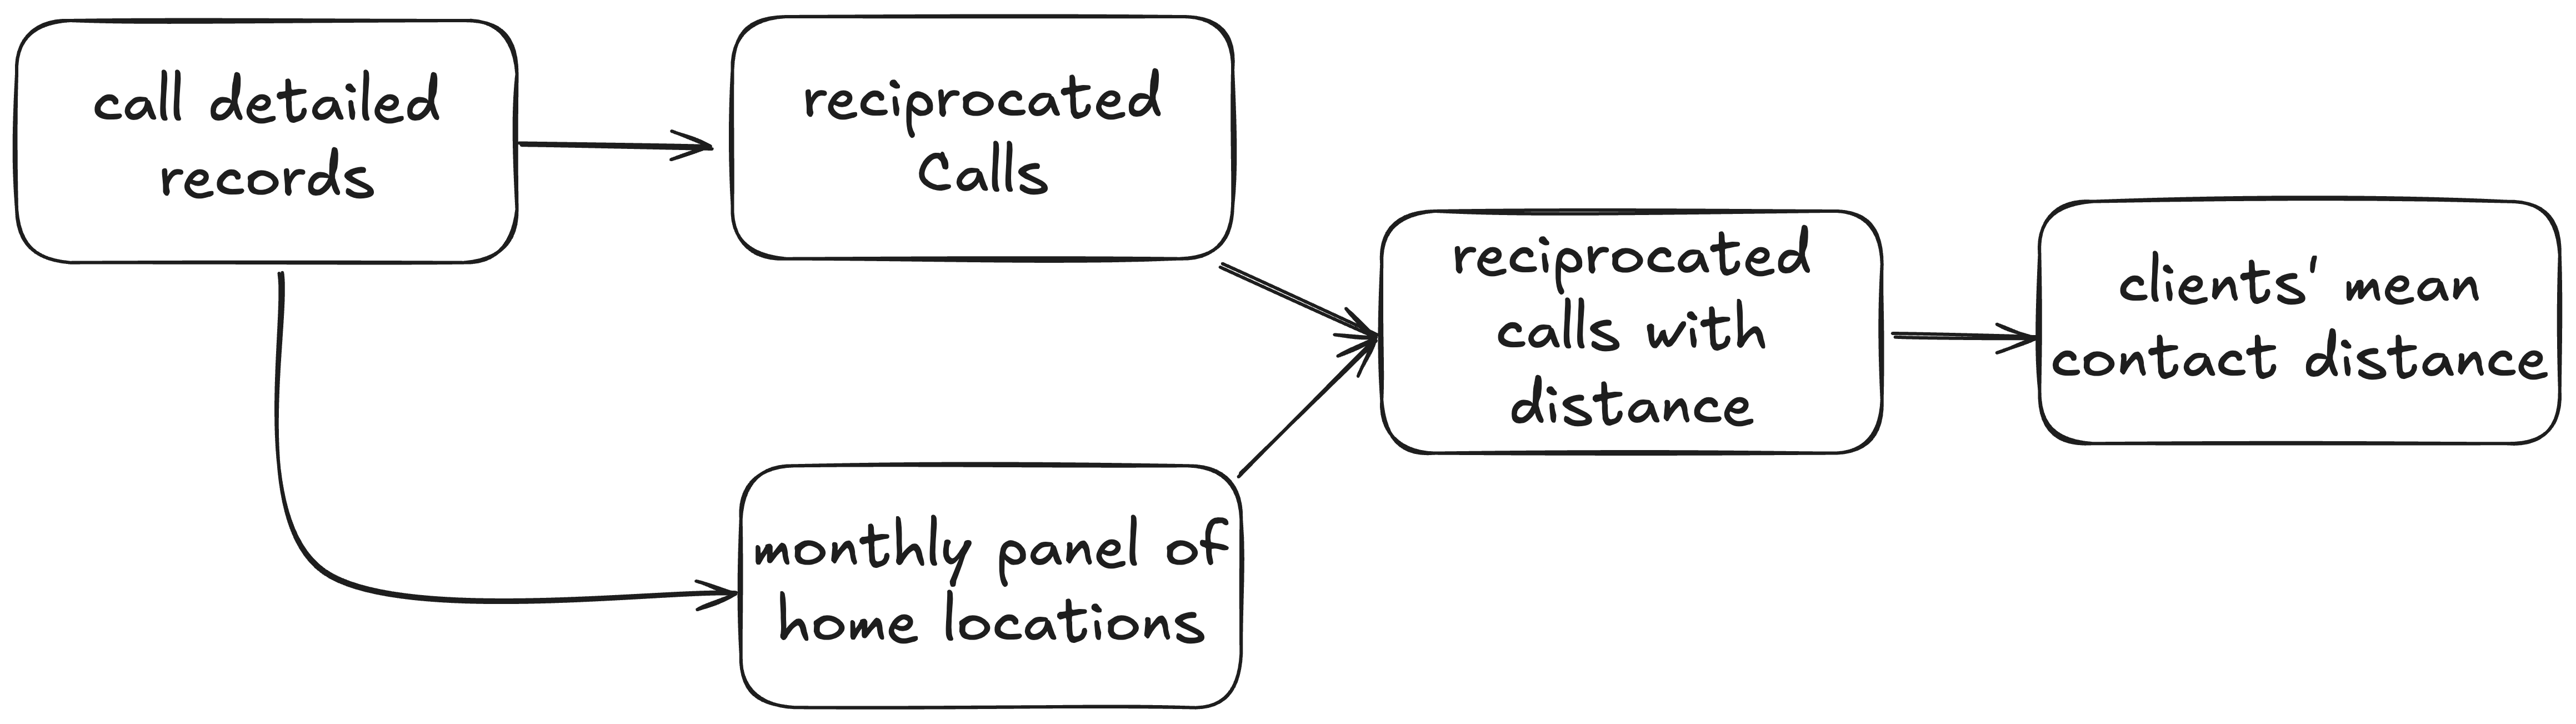
\includegraphics[scale=0.091]{figures/pipeline_mean_contact_distance.png}


% \caption*{Notes: .}
\label{fig:pipeline_contact_distance}
\end{figure}

Figure~\ref{fig:pipeline_contact_distance} demonstrates how to construct the contact distance for user $i$ in month $m$.
Note that the estimation of home location is necessary in our situation as we do not have the geographical locations of both the caller and recipient for each call; instead, only a single location is attached to each phone call---specifically from one telecom base station (see Table~\ref{tab:example_cdr}).
Therefore, we impute these locations using the corresponding home locations obtained through our proposed estimation approach.
Furthermore, as the home location for a given month is estimated through CDRs, the estimation will fail for some months that lack CDRs.
We employ forward imputation followed by backward imputation to address this issue. Forward imputation means using month $m-1$ to impute month $m$'s home location (if month $m$ doesn't have any CDR), while backward imputation uses month $m+1$ to impute month $m$'s home location.

\begin{definition}[Outgoing Contact Distance]
The outgoing contact distance \( cd^{\text{out}}_{i, m} \) (where $cd$ stands for contact distance) for user $i$ in month $m$ is defined by:
\[
cd^{\text{out}}_{i, m}
=
\sum_{j \in V^{\text{out}}_{i, m} } \hat{p}_{i, j, m}
\cdot
d(\text{home}_{i, m}, \text{home}_{j, m})
\]
where $V^{\text{out}}_{i, m}$ and $\hat{p}_{i, j, m}$ is defined in Equation~\ref{eq:outgoing_contacts} and ~\ref{eq:weight_j_for_i_in_month_m}, respectively. $d$ is the measure of geographic distance between two coordinates, and $\text{home}_{i, m}$ represents the home coordinates for user $i$ in month $m$.
\end{definition}

\nameref{appendix_event_centered_trends} demonstrates time series for two groups of features, showing the mean for the treated group against that of the untreated group, with all data points subtracted from the mean in the reference period. This allows us to better examine the outcome trends in both pre-treatment and post-treatment periods.


\clearpage\newpage
\subsection{Human Mobility Features}
Numerous studies have used CDRs to analyze human mobility patterns. We largely follow the literature in constructing mobility features but determine the weight of a telecom base station for a phone user by temporal size (see Equation~\ref{eq:temporal_size}) rather than call count, which corrects distortion caused by routing mechanisms. We use notations similar to those in Section~\ref{sec:notations} to avoid redundant redefinition.

There are two key differences. First, we now use CDRs from weekdays, including both daytime and nighttime records. Second, we add a monthly dimension, constructing features on a monthly basis. For example, $B_{i, m} \subset B$ denotes the collection of telecom base stations that handled calls for user $i$ in month $m$, $R_{i, m, b} \subset R$ represents call records that are related to user $i$ in month $m$ and associated with base station $b \in B_{i, m}$, and $T_{i, m, b} \subset T$ denotes timestamps connected to $R_{i, m, b}$.

Human mobility features are derived purely from CDRs, with the locations of telecom base stations serving as proxies for visited places. Therefore, all geographic information is represented by a location matrix $L^{\text{geo}}_{i, m}$ defined as follows.

\begin{definition}[Geographic Location Matrix]
A geographic location matrix $L^{\text{geo}}_{i, m} \in \mathbb{R}^{\lvert B_{i, m} \rvert \times 2}$ contains all visited coordinates for user $i$ in month $m$, where the two columns record the longitude and latitude, respectively, of each telecom base station $b \in B_{i, m}$.
Besides, we denote $(l^\text{geo}_{i, m})_b \in \mathbb{R}^2$ as the row of $L^\text{geo}_{i, m}$ that corresponds to telecom base station $b \in B_{i, m}$, which contains the longitude and latitude information of that telecom base station.
\end{definition}

Mobility features often lay on the foundation of empirical probability distribution over the visited locations (rows of the location matrix). As mentioned, we consider a new weighting scheme where the weight for each $b \in B_{i, m}$ is defined as the temporal size $\mu(T_{i, m, b})$, and therefore, the corresponding empirical probability is given by:
\begin{equation}
\hat{p}^{\mu}_{i, m, b}
=
\frac{\mu(T_{i, m, b})}{\sum_{b' \in B_{i, m}} \mu(T_{i, m, b'})}
\end{equation}
in contrast to the traditional approach:
\begin{equation}
\hat{p}^{T}_{i, m, b}
=
\frac{\lvert T_{i, m, b} \rvert}{\sum_{b' \in B_{i, m}} \lvert T_{i, m, b'} \rvert}.
\end{equation}
Note that in the following text, we will operate on the empirical probability vector $\hat{p}_{i, m} \in \mathbb{R}^{\lvert B_{i, m} \rvert}$, where each entry $\hat{p}_{i, m, b}$ corresponds to the empirical probability of base station $b \in B_{i, m}$ and can be computed using either the temporal size approach ($\hat{p}^{\mu}_{i, m, b}$) or the traditional call count approach ($\hat{p}^{T}_{i, m, b}$).

Geographic distance (geodesic distance) on the Earth's surface differs from Euclidean distance calculated directly from longitude-latitude coordinates, as the former accounts for spherical geometry while the latter assumes a flat coordinate space.
To make spatial statistical analysis meaningful, we employ the Azimuthal Equidistant (AEQD) projection centered at the geographic mean of locations $(r_c)^{\text{geo}}_{i, m}$, which is given by:
\begin{equation}
(r_c)^{\text{geo}}_{i, m}
=
(L^{\text{geo}}_{i, m})^{'} \hat{p}_{i, m}
\in \mathbb{R}^2.
\end{equation}
This projection ensures that Euclidean distances from the projection center to any point correspond to actual geographic distances from the geographic centroid.
This makes variance-covariance matrices computed on the projected coordinates geographically interpretable, as they accurately reflect the spatial spread of locations around their geographic center. Besides, we denote $L_{i, m}$, $(l_{i, m})_b$, and $(r_c)_{i, m}$ as the projected location matrix, the projected coordinates of a telecom base station, and the projected centroid, respectively.

After completing the preliminary setup, we can now construct mobility features that aim to measure: (i) how large the activity area is (radius of gyration), (ii) how unpredictable spatial movement patterns are (movement entropy), and (iii) to what extent the activity area spreads in an elliptical shape (eccentricity), which indicates whether a user visits locations primarily along a fixed direction.

\begin{definition}[Radius of Gyration]
The radius of gyration $(r_g)_{i, m}$ for user $i$ in month $m$ is defined by:
\[
(r_g)_{i, m}
=
\sqrt{
    \kappa_{i, m}
    \sum_{ b \in B_{i, m}}
    \hat{p}_{i, m, b} \cdot \lVert (l_{i, m})_b - (r_c)_{i, m} \rVert^2
},
\]
where $\kappa_{i, m}$ is the bias-correction factor.
\end{definition}


Note that:
\[
\kappa_{i, m}
=
\frac{
\sum_{b \in B_{i, m}}
    \mu(T_{i, m, b})
}{
\left (
    \sum_{b \in B_{i, m}}
        \mu(T_{i, m, b})
\right )
-
1
}
\]
if $\hat{p}_{i, m, b} = \hat{p}^{\mu}_{i, m, b}$, else:
\[
\kappa_{i, m}
=
\frac{
    \sum_{b \in B_{i, m}}
        \lvert T_{i, m, b} \rvert
}{
    \left (
        \sum_{b \in B_{i, m}}
            \lvert T_{i, m, b} \rvert
    \right )
    -
    1
}.
\]

\begin{definition}[Movement Entropy]
The movement entropy $me_{i, m}$, where $me$ stands for movement entropy, for user $i$ in month $m$ is defined by:
\[
me_{i, m}
=
\frac{
- \sum_{b \in B_{i, m}}
    \hat{p}_{i, m, b}
    \log(\hat{p}_{i, m, b})
}{
\log(\lvert B_{i, m} \rvert )
}.
\]
\end{definition}

\clearpage\newpage
\begin{definition}[Eccentricity]
Given $\hat{\Sigma}_{i, m}$ is the sample variance-covariance matrix of $L_{i, m}$, eccentricity $ecc_{i, m}$, where $ecc$ stands for eccentricity, for user $i$ in month $m$ is defined as:
\[
ecc_{i, m}
=
\sqrt{
    1
    -
    \left(
        \frac{\lambda_{1}}{\lambda_{2}}
    \right)^2
}
\]
where $\lambda_{1}$ is the major eigenvalue of $\hat{\Sigma}_{i, m}$ and $\lambda_{2}$ is the minor one.
\end{definition}

The sample variance-covariance matrix $\hat{\Sigma}_{i, m}$ is constructed in two steps.
First, compute the demeaned location matrix:
\[
\tilde{L}_{i, m}
=
L_{i, m}
-
\mathbf{1}\hat{\mu}_{i, m}^{'}
\]
where $\mathbf{1} \in \mathbb{R}^{\lvert B_{i, m} \rvert }$ is a vector of ones and $\hat{\mu}_{i, m}$ is the sample mean, which is equivalent to $(r_c)_{i, m}$.
Then, the sample variance-covariance matrix is defined by:
\[
\hat{\Sigma}_{i, m}
=
\kappa_{i, m} (
    \tilde{L}_{i, m}'
    \text{Diag}(\hat{p}_{i, m})
    \tilde{L}_{i, m}
)
\]
where $\text{Diag}(\hat{p}_{i, m})$ is a diagonal matrix with the probability weights $\hat{p}_{i, m}$ on its diagonal, and $\kappa_{i, m}$ is the bias-correction factor.
This $2\times2$ matrix captures the spatial dispersion pattern, with eigenvalues determining the major and minor axes of the elliptical distribution.

\clearpage\newpage
\section{Empirical Strategy}
In this section, we introduce the concept of potential outcome framework and the average treatment effect on the treated (ATT) to formalize our research question.
As a straightforward and ideal definition, ATT provides clear guidance on what should be estimated.
Moreover, our empirical strategy to estimate ATT is through the extended Difference-in-Differences (DiD) design.
Subsequently, we elaborate on what estimation approach we adopt and the corresponding motivations.
The estimation approach comes with various possible setups, and we explain which are the most suitable for us.

% \textbf{Q: What empirical strategy do you use? Why do you use it?}

As we are interested in the effects of residential shifts and smartphone adoption on human mobility patterns and mobile communication behaviors, we formalize our research questions as follows: What are the magnitudes of differences in mobility and communication behaviors for individuals who receive these treatments compared to a counterfactual scenario where they never experienced them?
We define treatments as either residential shifts or smartphone adoption events. Given that many individuals in our sample receive the treatment, it is natural to focus on average treatment effects rather than individual-level effects. Moreover, since our primary interest lies in understanding how these life events specifically impact those who experience them---addressing the counterfactual question "what would have happened if they had not been treated?"---we focus on ATT as our primary causal parameter of interest.
Furthermore, examining how ATT evolves over time provides an additional dimension for analysis, and given these motivations, DiD with the design of multiple periods (also known as the event study) is an ideal econometric approach for examining both the ATT and its temporal dynamics.

% \textbf{For some of those who are not familiar with DiD, give a brief introduction}

The intuition of DiD is that simply comparing treated and untreated units at a single point in time may be misleading because these groups might differ in unobservable ways. Similarly, comparing the same units before and after treatment might confound the treatment effect with general time trends that would have occurred regardless of treatment.

DiD solves this problem by using a "double comparison." Suppose the treatment occurs in time period \( t \), and first, it compares the change in outcomes for the treated group over time:
\[
\mathbb{E}[Y_{i, t} - Y_{i, t-1} \mid D_i = 1]
\]
where \( D_i \) is a binary variable indicating whether an individual \( i \) is treated. Second, it compares this change to the change observed in a control group over the same period:
\[
\mathbb{E}[Y_{i, t} - Y_{i, t-1} \mid D_i = 1]
-
\mathbb{E}[Y_{i, t} - Y_{i, t-1} \mid D_i = 0]
\]
The key assumption is that, in the absence of treatment, both groups would have experienced the same time trend, where is called the parallel trends assumption (hereafter PTA).
Under this assumption, any difference in the trends between the two groups can be attributed to the ATT.

Note that the above example represents the canonical \( 2 \times 2 \) DiD design, which involves exactly two groups and two time periods.
To examine treatment effect dynamics across multiple time periods, we can generalize this approach by selecting a reference period, which is \( t-1 \) in the above example, and applying the DiD logic to estimate treatment effects for each subsequent period relative to the predefined reference period.
Furthermore, the canonical \( 2 \times 2 \) setup assumes static treatment timing, where all treated units receive treatment simultaneously. However, our empirical setting are different in the sense that treatment units become treated at different periods. This variation in treatment timing introduces additional complexity, and several econometrics tools have proposed to address this issue.

% \textbf{Put the focus on the staggered DiD and provide a stylized fact by checking the outcomes' evolution paths}

In the Definition \ref{def:migrants}, we include treatment units with staggered treatment adoption to avoid contemporaneous confounders, leading to a robust estimation.
However, the design of DiD with multiple periods and staggered treatment adoption, through two-way fixed effect specification may be biased due to the forbidden comparison (this term also used by \cite{roth2023s} and \cite{de2023two}). That is, comparing the latter treated units to the early treated units, in the context of time-variant treatment effects (\cite{goodman2021difference}, \cite{sun2021estimating}, \cite{baker2022much}).
Through inspecting how mobility and mobile communication features evolve after residential shift (see Figure from \ref{fig:effect_of_residential_shift_on_total_duration} to \ref{fig:effect_of_residential_shift_on_temporal_size_weighted_count_weighted_eccentricity}) and smartphone adoption (see Figure from \ref{fig:effect_of_smartphone_adoption_on_outgoing_incoming_total_duration} to \ref{fig:effect_of_smartphone_adoption_on_temporal_size_weighted_count_weighted_eccentricity}), we can observe the non-static treatment effect dynamics, resulting in the inapplicability of two-way fixed effects models.

Consequently, we follow the estimation approach proposed by \cite{callaway2021difference}, which estimates the ATT dynamics for each treatment-timing cohort independently with the valid control group, thereby avoiding the issue of forbidden comparison.
Note that aside from \cite{callaway2021difference}, many other econometric tools have been proposed to solve the issue as to the forbidden comparison, and \cite{roth2023s} and \cite{de2023two} both provide comprehensive introduction and briefly summarize the differences across various approaches.
We choose \cite{callaway2021difference} over other alternatives as it's considered to be more flexible in (i) the selection of valid control units, (ii) the aggregation of estimated treatment effects across cohorts and periods, and (iii) the assumption on parallel trends.

% \begin{equation}
% Y_{i, m} = \alpha_i + \lambda_m + \Sigma_{b \in \mathcal{B}} \delta_{b} \cdot \mathbbm{1}[m - E_i = b] \times D_i + \epsilon_{i, m}
% \end{equation}
% where $Y_{i, m}$ is the outcome, $\alpha_i$, $\lambda_m$ are individual and time fixed effects, respectively, $\delta_b$ is the treatment effect at relative period $b$, $\mathcal{B}$ is the set of relative periods, defined as $\mathcal{B} := \{-3, -2, 0, \ldots, 3\}$, $E_i$ is the treatment timing, $D_i$ is the treatment indicator, equaling to 1 if $i$ is a treated unit and 0 otherwise, and $\epsilon_{i, m}$ is the error term.

% \textbf{Q: What's the summary of your empirical strategy? Any suggestions from the authors who propose this idea? Do you follow? Why or why not?}

\cite{callaway2021difference} name the ATT specific to a period and treatment-timing cohort as group-time ATT where the group is defined as the treatment-timing cohort.
Therefore, in the following text, "groups" refers to treatment-timing cohorts while "cohorts" aside from groups, the control units are included as a single cohort.

As mentioned, the key point of dealing with the time-variant treatment effects with staggered treatment adoption is to employ valid control units.
\cite{callaway2021difference} is flexible in the selection of valid control units in the sense that they allow either the never-treated units or the not-yet-treated units to be control units depending on the practitioners' need. However, others' control units (e.g., \cite{sun2021estimating} and \cite{borusyak2024revisiting}) encompass of both never-treated and not-yet treated units, and don't have the freedom to choose either of them. Despite flexible, \cite{callaway2021difference} suggest employing the early-treated samples as the comparison only if the never-treated units are unavailable or limited in size. In our situation where only a small fraction of samples decides to change their homes or start using smartphones, never-treated samples are quite suitable as the comparison.

\cite{callaway2021difference} aim at estimating ATT for each group and period, and therefore, researcher has the full customizability to aggregate them across groups and periods to obtain a summary ATT.
Additionally, they incorporate covariates on which PTA conditions, which should be reasonable when the unconditional PTA is violated because groups differ in observable characteristics that affect outcome trends.
Nevertheless, conditional PTA introduces additional layer of complexity for estimation, so we will first start from the unconditional version for estimation, and if we clearly see the patterns of violation, we will move to incorporate the pre-treatment covariates, adopting the conditional PTA.

Furthermore, the anticipation is allowed, which is particularly useful when discussing the impacts of residential shift as mobility or mobile communication features might start to change prior to the actual relocation timing due to exploring potential neighborhoods, researching local amenities, or establishing new social connections. Lastly, given the non-parametric nature of \cite{callaway2021difference}'s approach, the inference is done through a bootstrap process to obtain confidence intervals.

\section{Group-Time ATT}
Before introducing the group-time ATT, we need to set up the potential outcome framework first to let the ATT have a clearer definition.
Since we include treatment units with four different treatment timings and if treatment effects are effective and heterogeneous across treatment-timing cohorts, we can observe five different aggregated outcome paths as shown in previous section. Therefore, for each user $i$, in each month $m \in \mathcal{M}$, there will be 5 potential outcomes: $Y_{i, m}(\infty)$, $Y_{i, m}(4)$, $Y_{i, m}(5)$, $Y_{i, m}(6)$, and $Y_{i, m}(7)$. $Y_{i, m}(\infty)$ is the potential outcome in month $m$ for user $i$ if $i$ has never received the treatment throughout the sample period. In our case, phone users are considered to be treated if they either relocation or switch to smartphone. $Y_{i, m}(g)$ where $g \in \{4,5,6,7\}$ is the potential outcome in month $m$ for user $i$ if $i$ is treated in month $g$ ($i \in \mathcal{G}_g$). For each user $i$ and month $m$, only 1 potential outcome can be realized, becoming observable. Hence, the connection between potential outcomes and the observed outcome $Y_{i, m}$ is established (\cite{callaway2021difference}, \cite{sun2021estimating}) as follows:
\begin{equation}\label{eq:observed_outcome}
Y_{i, m}
= Y_{i, m}(\infty)
    + \Sigma_{g=4}^7 ( Y_{i, m}(g) - Y_{i, m}(\infty) ) \cdot G_{i, g}
\end{equation}
where $G_{i, g}$ is a binary variable defined as:
$$
G_{i, g} =
\begin{cases}
    1,
    & \text{if } i \in \mathcal{G}_g \text{, i.e., $i$ receives the treatment in month $g$} \\
    0,
    & \text{otherwise}.
\end{cases}
$$
Besides, we define an additional binary variable for indicating whether $i$ is in the never-treated cohort $g_\infty$:
$$
G_{i, \infty} =
\begin{cases}
    1,
    & \text{if } i \in \mathcal{G}_{\infty} \\
    0,
    & \text{otherwise}.
\end{cases}
$$

Anticipation is a critical topic when estimating the ATT as it determines which pre-treatment period is considered as the reference to correctly assess treatment effects. Let $\delta$ be the number of anticipation months, and for cohort $\mathcal{G}_g$, $g-\delta$ becomes the cutoff value (note that if $\delta=0$, the cutoff value is $g$, which returns to the conventional setting) and treatment effect dynamics are inspected for each month $m >= g-\delta$, as treatment effects are expected to let $Y_{i, m}(g)$ deviate from $Y_{i, m}(\infty)$ starting at any timing $m$ after $g-\delta$. This also implies:
\begin{equation}\label{eq:equivalence_potential_outcome}
    Y_{i, m}(g) = Y_{i, m}(\infty)
\end{equation}
for all $i \in \mathcal{G}_g$ and $m < g - \delta$ (modified from the Assumption 5 in \cite{roth2023s}). If we jointly consider the equation \ref{eq:observed_outcome} and \ref{eq:equivalence_potential_outcome}, we can further derive:
\begin{equation}\label{eq:equivalence_observed_outcome_pretreatment}
    Y_{i, m} = Y_{i, m}(g) = Y_{i, m}(\infty)
\end{equation}
for all $i \in \mathcal{G}_g$ and $m < g - \delta$.

With these potential outcome notations, it's time to define the ATT, which discusses the effects of a treatment in the counterfactual sense.

\begin{definition}[Group-Time ATT]\label{def:ATTgt}
The ATT specific to treatment-timing cohort $\mathcal{G}_g$ in month $m \in \mathcal{M}$ is defined as:
$$
ATT(g, m)
= \mathbb{E}[Y_{i, m}(g) - Y_{i, m}(\infty) \mid G_{i, g} = 1],
$$
which is the expected difference between potential outcomes in month $m$ for cohort $\mathcal{G}_g$.
\end{definition}

As user $i$ belongs to the cohort $\mathcal{G}_g$, by equation \ref{eq:observed_outcome}, we know $Y_{i, m}(g)$ is observable and equivalent to $Y_{i, m}$. Therefore, the group-time ATT can be rewritten as:
\begin{align}\label{def:ATTgt_v2}
ATT(g, m)
&=
\mathbb{E}[
    Y_{i, m} - Y_{i, m}(\infty)
    \mid G_{i, g} = 1
]
\nonumber \\
&=
\mathbb{E}[
    Y_{i, m}
    \mid G_{i, g} = 1
]
-
\mathbb{E}[
    Y_{i, m}(\infty)
    \mid G_{i, g} = 1
],
\end{align}
which is the difference between the expected observed outcome $Y_{i, m}$ with respect to cohort $\mathcal{G}_g$ and the expected potential outcome in month $m$ that would occur if they have never been exposed to the treatment.

Note that notations in Definition \ref{def:ATTgt} are a little bit different from \cite{callaway2021difference} in the way that they denote the period as $t$ and causal parameter as $ATT(g, t)$ while we use $m$ to emphasize the monthly periods. Besides, we also replace the 0 with $\infty$ used by \cite{sun2021estimating} and \cite{borusyak2024revisiting} to align the meaning of never-treated units, which become treated at some point in the infinite future.

Given the anticipation months $\delta$, and considering a treatment-timing cohort $\mathcal{G}_g$, for each $m \geq g-\delta$, $Y_{i, m}(\infty)$ is unobservable. Therefore, we need an assumption to make $ATT(g, m)$ identifiable for month $m \geq g-\delta$, and that's where PTA comes into play.

\begin{definition}[Parallel Trend Assumption]\label{def:parallel_trend}
Given the number of anticipation months $\delta$, for each $\mathcal{G}_g$ where $g \in \{4,5,6,7\}$ and $m \geq g-\delta$, the following equality is assumed:
\begin{equation}\label{eq:parallel_trend}
\mathbb{E}[ Y_{i, m}(\infty) - Y_{i, m-1}(\infty) \mid G_{i, g} = 1]
= \mathbb{E}[ Y_{i, m}(\infty) - Y_{i, m-1}(\infty) \mid G_{i, \infty} = 1 ].
\end{equation}
\end{definition}

That is, for all group $\mathcal{G}_g$ and month $m \geq g-\delta$, the trend in the counterfactual outcome of never-treated measured between month $m$ and $m-1$ should be expectedly identical between group $\mathcal{G}_g$ and the never-treated cohort $\mathcal{G}_{\infty}$ for all $\mathcal{G}_g$.
It's an assumption as objects in the equality are potential outcomes $Y_{i, m}(\infty)$, which are clearly unobservable in the post-treatment periods for all $\mathcal{G}_g$. As mentioned, we will impose the unconditional PTA first, and switch to the conditional version if needed.
% For the derivation of how the conditional PTA can facilitate the estimation of ATT, please refer to the original paper or quickly scan through \nameref{pta_att}, which provides a short introduction based on my personal understanding.
% \cite{callaway2021difference} claim that the conditional PTA is more realistic as the unconditional PTA can be easily violated if the outcome trend is determined by covariates:
% \[
% \mathbb{E}[Y_{i, m}(\infty) - Y_{i, m-1}(\infty) \mid X_i],
% \]
% and the covariate distribution is imbalanced between \( \mathcal{G}_g \)	 and the control group:
% \begin{align*}
% &\mathbb{E}[Y_{i, m}(\infty) - Y_{i, m-1}(\infty) \mid G_{i, g} = 1]
% \\
% &=
% \mathbb{E}_{X_i \mid G_{i, g=1}}[\mathbb{E}[Y_{i, m}(\infty) - Y_{i, m-1}(\infty) \mid X_i]]
% \\
% &\neq
% \mathbb{E}_{X_i \mid G_{i, \infty=1}}[\mathbb{E}[Y_{i, m}(\infty) - Y_{i, m-1}(\infty) \mid X_i]]
% \\
% &=
% \mathbb{E}[Y_{i, m}(\infty) - Y_{i, m-1}(\infty) \mid G_{i, \infty} = 1].
% \end{align*}
% Therefore, conditional PTA is more robust when groups differ in observable characteristics that affect outcome trends. Moreover, if the unconditional PTA already holds, it means the parallel trends assumption is satisfied without conditioning on any covariates. In this case, adding covariates to make it "conditional" shouldn't change the core identification.

% Besides, although the assumption is required to hold in all month $m \in \mathcal{M}$, it can actually be assumed to hold only in post-treatment periods ($m \geq g-\delta$) since \( Y_{i, m}(\infty) \) where \( m < g-\delta \)	is observable and equal to the observed outcome \( Y_{i, m} \).

The parallel trend assumption stated in Definition \ref{def:parallel_trend} is employed in the canonical $2 \times 2$ DiD design, and it's necessary to extend it for the multiple periods case, which is given by:
\begin{equation}\label{eq:parallel_trend_general_first}
\mathbb{E}[Y_{i, m}(\infty) - Y_{i, g-\delta-1}(\infty) \mid X_i, G_{i, g} = 1]
=
\mathbb{E}[Y_{i, m}(\infty) - Y_{i, g-\delta-1}(\infty) \mid X_i, G_{i, \infty} = 1],
\end{equation}
and it can be further simplified to:
\begin{equation}\label{eq:parallel_trend_general}
\mathbb{E}[Y_{i, m}(\infty) - Y_{i, g-\delta-1} \mid X_i, G_{i, g} = 1]
=
\mathbb{E}[Y_{i, m} - Y_{i, g-\delta-1} \mid X_i, G_{i, \infty} = 1].
\end{equation}
Equation \ref{eq:parallel_trend_general_first} can be obtained from Equation \ref{eq:parallel_trend} by adding all parallel trend equality in post-treatment periods and by the end, $Y_{i, g-\delta-1}(\infty)$ appears, which is observable since $Y_{i, g-\delta-1}(\infty) = Y_{i, g-\delta-1}$. As mentioned in \cite{roth2023s}, for the ATT in the longer periods after treatment to be identifiable, a stronger assumption needs to be imposed.

With equation \ref{eq:parallel_trend_general}, $\mathbb{E}[Y_{i, m}(\infty) \mid G_{i, g} = 1]$ becomes identifiable:
\begin{align}
\mathbb{E}[Y_{i, m}(\infty) \mid G_{i, g} = 1]
&=
\mathbb{E}[Y_{i, g-\delta-1}(\infty) \mid G_{i, g} = 1]
\nonumber \\
&\quad\quad
+\mathbb{E}[Y_{i, m}(\infty) \mid G_{i, g} = 1]
    - \mathbb{E}[Y_{i, g-\delta-1}(\infty) \mid G_{i, g} = 1]
\nonumber \\
&=
\mathbb{E}[Y_{i, g-\delta-1} \mid G_{i, g} = 1]
\nonumber \\
&\quad\quad
+\mathbb{E}[Y_{i, m} \mid G_{i, \infty} = 1]
- \mathbb{E}[Y_{i, g-\delta-1} \mid G_{i, \infty} = 1]
\nonumber \\
&=
\mathbb{E}[Y_{i, g-\delta-1} \mid G_{i, g} = 1]
+
\mathbb{E}[Y_{i, m} - Y_{i, g-\delta-1} \mid G_{i, \infty} = 1],
\end{align}
Then, group-time ATT can be derived by:
\begin{align} \label{eq:att_gt_full}
ATT(g, m)
&=
\mathbb{E}[
    Y_{i, m}
    \mid G_{i, g} = 1
]
-
\mathbb{E}[
    Y_{i, m}(\infty)
    \mid G_{i, g} = 1
]
\nonumber \\
&=
\mathbb{E}[
    Y_{i, m}
    \mid G_{i, g} = 1
]
\nonumber \\
&\quad\quad
- \mathbb{E}[Y_{i, g-\delta-1} \mid G_{i, g} = 1]
-
\mathbb{E}[Y_{i, m} - Y_{i, g-\delta-1} \mid G_{i, \infty} = 1]
\nonumber \\
&=
\mathbb{E}[Y_{i, m} - Y_{i, g-\delta-1} \mid G_{i, g} = 1]
-
\mathbb{E}[Y_{i, m} - Y_{i, g-\delta-1} \mid G_{i, \infty} = 1]
\end{align}
By Equation \ref{eq:att_gt_full}, we can simply estimate $ATT(g, m)$ through its sample analogue. The simplicity credits to the unconditional PTA, and for how to incorporate conditional PTA, please refer to \cite{callaway2021difference}.

% Through this equation, we can see that $\mathbb{E}[Y_{i, m} - Y_{i, g-\delta-1} \mid G_{i, g} = 1]$ can be estimated through the sample analogue but $\mathbb{E}[Y_{i, m} - Y_{i, g-\delta-1} \mid X_i, G_{i, \infty} = 1]$ needs additional estimation, which is the identification strategy of the outcome regression.
% The performance of such estimation is not guaranteed, so \cite{abadie2005semiparametric} proposed a sample weighting scheme based on the inverse probability weighting (IPW) to avoid this estimation.
% The motivation is that since the need for estimation arises from the unbalanced covariate distribution between the two groups, \( \mathcal{G}g \) and \( \mathcal{G}_{\infty} \), we can design sample weights so that the covariate distributions match. However, since the weights is constructed based on the propensity scores, i.e., \( \mathbb{P}(G_{i, g} = 1 \mid X_i) \), we still need to estimate it.

% Both outcome regression and IPW rely on the correct modeling for conditional mean or propensity scores, respectively.
% That's where doubly-robust estimation comes into play, where it combines the outcome regression and the IPW, being robust if one of the model is correctly specified.
% Although the doubly robust estimation is more computationally demanding, as it needs to estimate two models compared to the others with each requiring one estimation, it is more robust so we follow the suggestion from \cite{callaway2021difference} to apply the doubly robust estimation for group-time ATT.


% \textbf{Q: Given its importance, can we test the PTA?}

It is important to note that PTA is extremely crucial for identification, as the ATT becomes unidentifiable without it. This raises the question whether there exists a method to test this assumption.
Typically, the assumption's plausibility is evaluated in the pre-treatment periods in an event study design. As in pre-treatment periods, the potential outcome of the never-treated $Y_{i, m}(\infty)$ is observable for all user $i$, and if the PTA holds in the pre-treatment periods, it might be relatively reasonable to claim that the parallel trend might also hold in post-treatment periods.

That's the reason why we plot the treated group's trajectories of mean outcomes centered at the reference period $g-\delta-1$, along with those of the control group. If in the pre-treatment periods, the treated group's trajectory highly overlaps with the control group's trajectory, it will be reasonable to claim that the parallel trend assumption holds in the pre-treatment periods. In all figures in \nameref{appendix_event_centered_trends}, we can see that the treated group's re-centered mean outcomes' trajectories highly overlaps with those associated to the control group's trajectory in the pre-treatment periods while with few exceptions occurring only in a particular treatment-timing cohort for some outcomes, which generally confirms the plausibility of parallel trend in pre-treatment periods.

Moreover, given that the treatment is not confounded, and anticipation effects are correctly accounted for, if PTA holds, the estimated ATT in pre-treatment periods should be statistically insignificant.
The intuition is that the treatment shouldn't take effects during pre-treatment periods and under PTA, treated units' outcome changes should be identical to the comparison group's changes over the same periods, yielding insignificant ATT estimation.
Therefore, by examining the estimation results in pre-treatment periods, we can assess whether the PTA holds during the pre-treatment periods.

% \textbf{Q: How to recover the event study from group-time ATT?}

After estimating the group-time ATT, we can recover the traditional event study through the following aggregation scheme provided by \cite{callaway2021difference}, which demonstrates the ATT after $e$ month of the treatment:
\begin{equation}\label{eq:event_aggregation}
\theta(e) = \sum_{g=4}^7 \mathbb{P}(G_{i, g} = 1) ATT(g, g+e) 1[g+e <= 10]
\end{equation}
where $\mathbb{P}(G_{i, g} = 1)$ is the group size of cohort $\mathcal{G}_g$ and $1[g+e <= 10]$ is an indicator function that equals to 1 if $g+e <= 10$ and 0 otherwise. Note that 10, representing May 2014, is the maximum month in our sample period. Moreover, we restrict $e$ to be from -3 to 3 to let the difference of $\theta(e)$ be the correct interpretation of treatment effect dynamics. The Intuition is within this event time interval, the share of group size of each treatment-timing cohort is fixed. For example, when $e=4$, the outcomes of cohort $\mathcal{G}_7$ are missing and when $e=-4$, the outcomes of cohort $\mathcal{G}_4$ are missing. For more details, please refer to the Equation 3.5 in \cite{callaway2021difference}.
